% Nội dung được chuyển đổi từ BBH BTL CNPM.pdf.

\begingroup

\sloppy

\setlength{\parindent}{1.2cm}

\setlength{\parskip}{0.35em}

\section{Mô tả dự án}
\subsection{Bối cảnh dự án và vấn đề}
Khu đô thị ĐHQG-HCM tập trung nhiều trường đại học, ký túc xá, thư viện và khu dịch vụ cộng đồng. Sinh viên học tập hoặc sinh sống trong khu đô thị có nhu cầu di chuyển giữa các trường, khu ký túc xá, khu dịch vụ và ga Metro ĐHQG bằng phương tiện điện cá nhân hoặc phương tiện điện dùng chung tại các Mobility Hub.

Nhu cầu di chuyển, đỗ xe và sạc biến động theo thời gian và theo từng khu vực, trong khi số lượng phương tiện, chỗ đỗ và cổng sạc tại mỗi Hub có giới hạn. Nếu các tài nguyên này không được theo dõi và điều phối phù hợp, có thể xảy ra tình trạng thiếu xe tại khu vực có nhu cầu cao, Hub quá tải, thiếu chỗ đỗ hoặc tăng thời gian chờ của người dùng.

Vì vậy, cần có một cơ chế quản lý và điều phối tập trung nhằm theo dõi trạng thái tài nguyên và hỗ trợ phân bổ chúng hiệu quả hơn trong toàn bộ mạng lưới Hub.

\setcounter{subsection}{1}

\subsection{Tổng quan hệ thống}

Trước những khó khăn trong việc quản lý và phân bổ tài nguyên, giải pháp được đề xuất là một hệ thống phần mềm hỗ trợ quản lý và điều phối mạng lưới Mobility Hub trong khu đô thị ĐHQG-HCM — Smart E-Mobility Hub. Hệ thống quản lý trạng thái gần thời gian thực của phương tiện điện dùng chung, chỗ đỗ xe, cổng sạc và mức độ sử dụng của từng Hub thông qua dữ liệu từ Bộ giả lập dữ liệu hoặc nguồn IoT trong tương lai.

Sinh viên có thể tìm kiếm Hub hoặc phương tiện phù hợp, xem trạng thái tài nguyên, đặt xe, đặt chỗ đỗ, nhận và trả phương tiện. Đối với phương tiện điện cá nhân, sinh viên có thể đăng ký nhu cầu sạc tại Hub. Các chức năng cần định danh được thực hiện thông qua tài khoản đã được xác thực bằng dịch vụ SSO.

Đơn vị vận hành được phân quyền để giám sát toàn bộ mạng lưới, xem cảnh báo quá tải, điều phối phương tiện, xử lý sự cố, xây dựng lịch sạc thông minh và thực hiện mô phỏng What-if. Kết quả mô phỏng được dùng để đánh giá phương án vận hành và không làm thay đổi trực tiếp trạng thái vận hành cơ sở.

\subsection{Các khái niệm nghiệp vụ và tài nguyên cốt lõi}

{
\small
\setlength{\tabcolsep}{3pt}
\renewcommand{\arraystretch}{1.25}
\begin{longtable}{|>{\raggedright\arraybackslash}p{4.0cm}|>{\raggedright\arraybackslash}p{8.8cm}|}
\hline
\textbf{Khái niệm} & \textbf{Ý nghĩa trong hệ thống} \\
\hline
\endfirsthead
\hline
\textbf{Khái niệm} & \textbf{Ý nghĩa trong hệ thống (tiếp theo)} \\
\hline
\endhead
Mobility Hub & Điểm tập trung xe điện, chỗ đỗ và cổng sạc tại ga Metro, ký túc xá, trường hoặc khu dịch vụ. \\
\hline
Phương tiện điện dùng chung & Xe đạp điện, xe máy điện hoặc phương tiện điện có thể được sinh viên đặt và sử dụng. \\
\hline
Phương tiện cá nhân & Xe điện của sinh viên; chỉ liên quan đến đặt chỗ đỗ và đăng ký/lập lịch sạc. \\
\hline
Chỗ đỗ & Một vị trí vật lý tại Hub, có trạng thái trống/đã đặt/đang sử dụng. \\
\hline
Cổng sạc & Tài nguyên sạc có trạng thái khả dụng/đang sạc/lỗi. \\
\hline
Trạng thái Hub & Mức độ sử dụng, số chỗ còn trống, số cổng sạc khả dụng và nguy cơ quá tải. \\
\hline
What-if Simulation & Chức năng giả lập các tình huống như phương tiện bị mất định vị, Hub quá tải sinh viên hoặc cổng sạc hỏng. \\
\hline
\end{longtable}
}

\noindent\textit{Ghi chú:} Nhân sự vận chuyển và đội kỹ thuật là các bộ phận nghiệp vụ thuộc Đơn vị vận hành. Họ nhận nhiệm vụ qua kênh nội bộ và không được mô hình hóa thành actor độc lập trong phạm vi đồ án.

\subsection{Các bên liên quan, vai trò và kỳ vọng}

{
\small
\setlength{\tabcolsep}{3pt}
\renewcommand{\arraystretch}{1.25}
\begin{longtable}{|>{\raggedright\arraybackslash}p{3.0cm}|>{\raggedright\arraybackslash}p{4.2cm}|>{\raggedright\arraybackslash}p{5.6cm}|}
\hline
\textbf{Bên liên quan} & \textbf{Vai trò đối với hệ thống} & \textbf{Kỳ vọng} \\
\hline
\endfirsthead
\hline
\textbf{Bên liên quan} & \textbf{Vai trò đối với hệ thống} & \textbf{Kỳ vọng (tiếp theo)} \\
\hline
\endhead
Sinh viên & Người dùng chính, sử dụng phương tiện dùng chung hoặc phương tiện cá nhân tại Hub. & Tìm và xem được tài nguyên gần thời gian thực; đặt xe/chỗ đỗ/sạc không bị trùng; nhận thông tin rõ ràng khi Hub đầy hoặc tài nguyên không khả dụng; dữ liệu cá nhân được bảo vệ. \\
\hline
Đơn vị vận hành & Vận hành mạng lưới Hub, theo dõi tài nguyên và xử lý tình huống. & Có dashboard tổng quan; nhận cảnh báo quá tải/sự cố; điều phối xe và lịch sạc; chạy mô phỏng mà không làm ảnh hưởng dữ liệu vận hành; truy vết được các thay đổi quan trọng. \\
\hline
Đơn vị sở hữu dịch vụ & Định hướng, đầu tư, đặt chính sách và đánh giá hiệu quả dịch vụ. & Tăng hiệu quả sử dụng xe, chỗ đỗ và cổng sạc; giảm mất cân bằng tài nguyên; có dữ liệu hỗ trợ quyết định mở rộng hoặc điều chỉnh dịch vụ. \\
\hline
\end{longtable}
}

\subsection{Mục tiêu dự án}

Các mục tiêu của dự án được đánh giá trong môi trường dữ liệu mô phỏng và các kịch bản kiểm thử do nhóm xác định.

{
\small
\setlength{\tabcolsep}{3pt}
\renewcommand{\arraystretch}{1.25}
\begin{longtable}{|>{\centering\arraybackslash}p{1.5cm}|>{\raggedright\arraybackslash}p{5.5cm}|>{\raggedright\arraybackslash}p{5.8cm}|}
\hline
\textbf{Mã} & \textbf{Mục tiêu cần đạt} & \textbf{Tiêu chí đánh giá khái quát} \\
\hline
\endfirsthead
\hline
\textbf{Mã} & \textbf{Mục tiêu cần đạt} & \textbf{Tiêu chí đánh giá khái quát (tiếp theo)} \\
\hline
\endhead
OBJ01 & Trong bộ kịch bản kiểm thử, ít nhất 90\% nhu cầu hợp lệ của Sinh viên tìm và đặt được tài nguyên đáp ứng tiêu chí. & Đo tỷ lệ nhu cầu hợp lệ hoàn thành thành công trong bộ kịch bản kiểm thử. \\
\hline
OBJ02 & Sau khi áp dụng phương án điều phối, số yêu cầu không được đáp ứng hoặc số Hub quá tải giảm ít nhất 20\% so với trước điều phối trong cùng kịch bản. & So sánh trạng thái trước và sau điều phối trên cùng dữ liệu, cùng kịch bản. \\
\hline
OBJ03 & 100\% tình huống quá tải/sự cố thuộc bộ kịch bản chuẩn tạo được cảnh báo và phương án xử lý. & Đối chiếu từng tình huống chuẩn với cảnh báo và phương án xử lý được tạo. \\
\hline
OBJ04 & Dữ liệu mô phỏng không ghi đè hoặc làm thay đổi trạng thái vận hành cơ sở. & So sánh trạng thái vận hành trước và sau mỗi lần mô phỏng. \\
\hline
OBJ05 & Không tạo đặt trùng khi thử nghiệm đồng thời; từ chối 100\% yêu cầu trái quyền. & Thực hiện kiểm thử đồng thời và kiểm thử phân quyền theo kịch bản xác định. \\
\hline
\end{longtable}
}

\subsection{Phạm vi và ranh giới hệ thống}

Smart E-Mobility Hub tập trung vào phần mềm quản lý và điều phối tài nguyên trong mạng lưới Mobility Hub thuộc khu đô thị ĐHQG-HCM.

\subsubsection{Trong phạm vi dự án}

\begin{itemize}

\item Quản lý thông tin và trạng thái của phương tiện điện dùng chung, chỗ đỗ, cổng sạc và mức độ sử dụng từng Hub; tiếp nhận dữ liệu cập nhật từ Bộ giả lập dữ liệu.

\item Hỗ trợ sinh viên tìm kiếm Hub và phương tiện phù hợp, xem trạng thái tài nguyên, đặt xe, nhận và trả phương tiện. Sinh viên sử dụng phương tiện cá nhân có thể đặt chỗ đỗ và đăng ký lịch sạc.

\item Hỗ trợ đơn vị vận hành giám sát mạng lưới, theo dõi tài nguyên, xem cảnh báo quá tải, điều phối phương tiện và xử lý sự cố.

\item Xây dựng lịch sạc thông minh dựa trên mức pin, nhu cầu sử dụng dự kiến và tình trạng tài nguyên sạc.

\item Mô phỏng các kịch bản What-if, đánh giá tác động và đề xuất phương án điều phối phù hợp.

\item Tích hợp SSO để xác thực người dùng, thực hiện phân quyền và lưu vết các thay đổi quan trọng.

\item Tích hợp dịch vụ bản đồ để hiển thị vị trí Hub và dịch vụ thông báo để chuyển các thông báo nghiệp vụ đến người dùng.

\item Cho phép tùy chỉnh chế độ giao diện mà không làm mất dữ liệu đang thao tác.

\end{itemize}

\subsubsection{Ngoài phạm vi dự án}

\begin{itemize}

\item Thiết kế, chế tạo, lắp đặt hoặc điều khiển trực tiếp phần cứng như xe điện, khóa xe, cảm biến và thiết bị sạc.

\item Triển khai mạng lưới IoT và hạ tầng vật lý thực tế; phiên bản dự án sử dụng dữ liệu giả lập để thể hiện trạng thái tài nguyên.

\item Tổ chức hoạt động vận chuyển, sửa chữa phương tiện hoặc xây dựng, mở rộng Hub ngoài thực tế; hệ thống chỉ hỗ trợ thông tin, lập phương án và ghi nhận trạng thái xử lý.

\end{itemize}

\subsubsection{Ranh giới hệ thống}

Hệ thống chịu trách nhiệm xử lý nghiệp vụ, quản lý dữ liệu, phân quyền, hiển thị thông tin và mô phỏng vận hành. Sinh viên và đơn vị vận hành tương tác với hệ thống từ bên ngoài. Dịch vụ SSO, Map API, dịch vụ thông báo và Bộ giả lập dữ liệu là các hệ thống ngoài trao đổi dữ liệu với Smart E-Mobility Hub; việc tích hợp các dịch vụ này thuộc phạm vi dự án, còn việc xây dựng chính các dịch vụ đó không thuộc phạm vi.

\subsection{Giả định, ràng buộc và các phụ thuộc bên ngoài}

\subsubsection{Các giả định ban đầu}

\begin{itemize}

\item Thông tin ban đầu về Hub, phương tiện, chỗ đỗ và cổng sạc được cung cấp đầy đủ; mỗi tài nguyên có mã định danh duy nhất.

\item Bộ giả lập dữ liệu cung cấp các bản tin theo định dạng đã thống nhất, có mã tài nguyên và thời điểm ghi nhận trạng thái.

\item Sinh viên và nhân viên vận hành có tài khoản hợp lệ trên dịch vụ SSO; hệ thống có thông tin để xác định vai trò và quyền truy cập tương ứng.

\item Các kịch bản kiểm thử có dữ liệu đầu vào xác định, bao gồm sức chứa Hub, số lượng tài nguyên, mức pin và nhu cầu sử dụng.

\item Việc đánh giá các chỉ tiêu hiệu năng được thực hiện trong môi trường kiểm thử có cấu hình và điều kiện mạng được ghi rõ.

\end{itemize}

\subsubsection{Các ràng buộc}

\begin{itemize}

\item Dự án triển khai ở mức phần mềm và sử dụng dữ liệu giả lập thay cho dữ liệu từ thiết bị IoT thực tế.

\item Bộ giả lập cung cấp dữ liệu trạng thái đầu vào; chức năng What-if sử dụng bản sao trạng thái vận hành để thử nghiệm các kịch bản. Hai hoạt động này có mục đích khác nhau.

\item Kết quả What-if không được tự động ghi đè hoặc làm thay đổi trạng thái vận hành cơ sở.

\item Việc đặt và phân bổ tài nguyên phải tuân thủ giới hạn sức chứa, tính khả dụng và các khoảng thời gian sử dụng, không tạo các lượt đặt xung đột.

\item Quyền truy cập và việc lưu vết thao tác phải tuân thủ các yêu cầu bảo mật đã xác định. Các chỉ tiêu chất lượng cụ thể được trình bày trong phần yêu cầu phi chức năng.

\end{itemize}

\subsubsection{Các phụ thuộc bên ngoài}

\begin{itemize}

\item Dịch vụ SSO: xác thực danh tính người dùng. Smart E-Mobility Hub sử dụng danh tính đã xác thực và thông tin vai trò để kiểm soát quyền truy cập.

\item Bộ giả lập dữ liệu: cung cấp dữ liệu về trạng thái phương tiện, mức pin, chỗ đỗ, cổng sạc và mức độ sử dụng Hub; mỗi gói tin có thời điểm phát sinh hoặc số phiên bản tại nguồn.

\item Map API: cung cấp chức năng bản đồ để hiển thị vị trí Hub, hỗ trợ người dùng tìm kiếm tài nguyên theo vị trí.

\item Dịch vụ thông báo: tiếp nhận yêu cầu gửi thông báo từ Smart E-Mobility Hub và chuyển thông tin đến người nhận tương ứng.

\end{itemize}

\subsection{Bảng tổng hợp truy vết}

{
\scriptsize
\setlength{\tabcolsep}{2pt}
\renewcommand{\arraystretch}{1.25}
\begin{longtable}{|>{\raggedright\arraybackslash}p{4.0cm}|>{\raggedright\arraybackslash}p{1.5cm}|>{\raggedright\arraybackslash}p{1.6cm}|>{\raggedright\arraybackslash}p{2.4cm}|>{\raggedright\arraybackslash}p{3.3cm}|}
\hline
\textbf{Nhu cầu/kỳ vọng} & \textbf{Mục tiêu} & \textbf{FR liên quan} & \textbf{Use Case liên quan} & \textbf{NFR liên quan} \\
\hline
\endfirsthead
\hline
\textbf{Nhu cầu/kỳ vọng} & \textbf{Mục tiêu} & \textbf{FR liên quan} & \textbf{Use Case liên quan} & \textbf{NFR liên quan (tiếp theo)} \\
\hline
\endhead
Sinh viên tìm được Hub/phương tiện phù hợp và xác định vị trí trên bản đồ. & OBJ01 & FR01, FR13 & UC1 & NFR01, NFR02 \\
\hline
Sinh viên xem trạng thái gần thời gian thực của phương tiện hoặc Hub. & OBJ01 & FR02 & UC2 & NFR02 \\
\hline
Sinh viên đặt xe dùng chung. & OBJ01, OBJ05 & FR03, FR14 & UC3 & NFR09, NFR10, NFR11, NFR12 \\
\hline
Sinh viên đặt chỗ đỗ xe. & OBJ01, OBJ05 & FR03, FR14 & UC4 & NFR09, NFR10, NFR11, NFR12 \\
\hline
Sinh viên nhận phương tiện đã đặt. & OBJ01 & FR03 & UC5 & NFR10, NFR11, NFR12 \\
\hline
Sinh viên trả phương tiện. & OBJ01 & FR03, FR14 & UC6 & NFR10, NFR11, NFR12 \\
\hline
Sinh viên đăng ký sạc. & OBJ01, OBJ02 & FR04 & UC7 & NFR09, NFR10, NFR11, NFR12 \\
\hline
Đơn vị vận hành giám sát mạng lưới. & OBJ02, OBJ03 & FR05 & UC8 & NFR02, NFR05, NFR10 \\
\hline
Đơn vị vận hành theo dõi tài nguyên. & OBJ02, OBJ03 & FR06 & UC9 & NFR02, NFR10 \\
\hline
Đơn vị vận hành xem cảnh báo quá tải. & OBJ02, OBJ03 & FR06, FR14 & UC10 & NFR02, NFR10 \\
\hline
Đơn vị vận hành điều phối phương tiện. & OBJ02, OBJ03 & FR07, FR14 & UC11 & NFR02, NFR09, NFR10, NFR11 \\
\hline
Đơn vị vận hành xử lý sự cố. & OBJ03 & FR07, FR14 & UC12 & NFR05, NFR10, NFR11 \\
\hline
Đơn vị vận hành xây dựng lịch sạc thông minh. & OBJ02 & FR09 & UC13 & NFR02, NFR08, NFR09, NFR10, NFR11 \\
\hline
Đơn vị vận hành mô phỏng phương án vận hành an toàn. & OBJ02, OBJ04 & FR08 & UC14 & NFR07, NFR10, NFR11 \\
\hline
Người dùng tùy chỉnh giao diện mà không mất dữ liệu đang thao tác. & OBJ01 & FR12 & UC15 & NFR13 \\
\hline
Trạng thái tài nguyên được cập nhật kịp thời và không bị dữ liệu lỗi thời ghi đè. & OBJ05 & FR10 & UC16 & NFR02, NFR05, NFR07, NFR08 \\
\hline
Người dùng được xác thực và chỉ truy cập chức năng, dữ liệu thuộc quyền. & OBJ05 & FR11 & UC17 & NFR10, NFR11 \\
\hline
NFR03: hiệu năng tải áp dụng toàn hệ thống. & Hỗ trợ toàn bộ mục tiêu & Không áp dụng trực tiếp & Toàn hệ thống & Kiểm thử tải và hiệu năng \\
\hline
NFR04: độ sẵn sàng áp dụng toàn hệ thống. & Hỗ trợ toàn bộ mục tiêu & Không áp dụng trực tiếp & Toàn hệ thống & Theo dõi uptime theo kỳ đo \\
\hline
NFR05: kháng lỗi áp dụng toàn hệ thống; thể hiện thêm ở UC8, UC12 và UC16. & Hỗ trợ toàn bộ mục tiêu & Không áp dụng trực tiếp & UC8, UC12, UC16; Toàn hệ thống & Fault-injection test \\
\hline
NFR06: sao lưu và phục hồi dữ liệu áp dụng toàn hệ thống. & Hỗ trợ toàn bộ mục tiêu & Không áp dụng trực tiếp & Toàn hệ thống & Kiểm thử sao lưu tại 00:00/12:00 và khôi phục trong tối đa 2 giờ \\
\hline
\end{longtable}
}

\section{Danh sách yêu cầu (Requirement Lists)}

\subsection{Yêu cầu chức năng (Functional requirements-FR)}

\subsubsection{Yêu cầu chức năng cho sinh viên}

\begin{itemize}

\item FR01: Hệ thống cho phép Sinh viên tìm kiếm phương tiện và Mobility Hub phù hợp dựa trên vị trí và các tiêu chí tìm kiếm.

\item FR02: Hệ thống cung cấp trạng thái gần thời gian thực của phương tiện và Hub, bao gồm mức pin, trạng thái xe, chỗ đỗ trống và cổng sạc khả dụng.

\item FR03: Hệ thống cho phép Sinh viên đặt xe, đặt chỗ đỗ, nhận xe và trả xe; không được tạo đặt trùng.

\item FR04: Hệ thống hỗ trợ Sinh viên đăng ký cổng sạc và khung giờ sạc cho phương tiện hợp lệ.

\end{itemize}

\subsubsection{Yêu cầu chức năng cho đơn vị vận hành}

\begin{itemize}

\item FR05: Hệ thống cung cấp dashboard để giám sát trạng thái và mức độ sử dụng của toàn bộ mạng lưới Mobility Hub.

\item FR06: Hệ thống phải phân tích trạng thái và mức độ sử dụng của các Hub để phát hiện Hub có nguy cơ quá tải, tạo và hiển thị cảnh báo cho Đơn vị vận hành, đồng thời cho phép theo dõi các tài nguyên liên quan.

\item FR07: Hệ thống hỗ trợ điều phối phương tiện giữa các Hub và xử lý các sự cố vận hành.

\item FR08: Hệ thống cho phép mô phỏng và phân tích kịch bản What-if trên dữ liệu cách ly, đồng thời đưa ra đề xuất điều phối.

\item FR09: Hệ thống hỗ trợ xây dựng lịch sạc thông minh dựa trên mức pin, thời điểm sử dụng dự kiến, thời gian chờ, trạng thái cổng sạc và sức chứa Hub; lịch phải xác định xe, cổng sạc, thời điểm bắt đầu/kết thúc và mức ưu tiên mà không tạo xung đột tài nguyên.

\end{itemize}

\subsubsection{Yêu cầu chức năng hệ thống và tích hợp}

\begin{itemize}

\item FR10: Hệ thống tiếp nhận, kiểm tra định dạng và cập nhật trạng thái từ Bộ giả lập dữ liệu theo thứ tự thời gian hoặc phiên bản.

\item FR11: Hệ thống tích hợp SSO để kiểm tra phiên, xác thực danh tính và phân quyền người dùng.

\item FR12: Hệ thống hỗ trợ thay đổi giao diện Sáng/Tối và ngôn ngữ mà không làm mất dữ liệu người dùng đang thao tác.

\item FR13: Hệ thống tích hợp Map API để hiển thị vị trí Hub và hỗ trợ Sinh viên tìm kiếm tài nguyên theo vị trí.

\item FR14: Hệ thống tạo nội dung thông báo và chuyển yêu cầu đến Hệ thống thông báo để phân phối cho UC3, UC4, UC6, UC10, UC11 và UC12 khi cần gửi ngoài ứng dụng.

\end{itemize}

\subsection{Yêu cầu phi chức năng (Non-Functional requirements-NFR)}

\subsubsection{Hiệu năng và Khả năng mở rộng (Performance \& Scalability)}

\begin{itemize}

\item NFR01: Hệ thống phải xử lý và phản hồi các yêu cầu tìm kiếm phương tiện/Mobility Hub phù hợp trong vòng tối đa 2.5 giây cho ít nhất 96\% số lượng truy vấn trong điều kiện mạng ổn định.

\item NFR02: Hệ thống phải cập nhật trạng thái thời gian thực (mức pin, vị trí đỗ, tình trạng Hub) trên giao diện người dùng không quá 15 giây kể từ khi nhận được gói dữ liệu IoT/mô phỏng mới.

\item NFR03: Với tải 15,000 phiên người dùng đồng thời theo workload kiểm thử đã mô tả, ít nhất 95\% request thuộc các chức năng tra cứu phải có thời gian phản hồi dưới 5 giây.

\end{itemize}

\subsubsection{Độ tin cậy và Tính sẵn sàng (Reliability \& Availability)}

\begin{itemize}

\item NFR04: Hệ thống phải đạt mức sẵn sàng tối thiểu 99.9\% theo tháng, không tính khoảng bảo trì đã thông báo trước từ 00:00 đến 04:00.

\item NFR05 (Sức chịu lỗi - Fault Tolerance): Sự cố mất kết nối hoặc hư hỏng tại một thiết bị hay một Mobility Hub đơn lẻ không được làm gián đoạn truy cập các Hub còn lại; Hub lỗi phải được đánh dấu không khả dụng.

\item NFR06: Hệ thống sẽ kích hoạt Cron job vào thời điểm 00:00 và 12:00 hằng ngày để tự động sao lưu toàn bộ dữ liệu của mạng lưới. Trong trường hợp xảy ra sự cố nghiêm trọng đối với cơ sở dữ liệu, hệ thống phải đảm bảo khả năng khôi phục trạng thái trong vòng tối đa 2 giờ đồng hồ.

\end{itemize}

\subsubsection{Tính toàn vẹn và Cách ly dữ liệu (Data Integrity \& Isolation)}

\begin{itemize}

\item NFR07: Dữ liệu và trạng thái sinh ra từ quá trình Mô phỏng (What-If Simulation) phải được cách ly hoàn toàn (Isolate) trên một môi trường ảo, tuyệt đối không được ghi đè hay làm ảnh hưởng đến dữ liệu của mạng lưới đang vận hành thực tế.

\item NFR08: Mỗi gói cập nhật phải chứa thời điểm phát sinh hoặc số phiên bản tại nguồn. Hệ thống phải từ chối và ghi log gói có thời điểm/số phiên bản không mới hơn trạng thái đang lưu của cùng tài nguyên.

\item NFR09 (Kiểm soát đồng thời): Trong mọi tình huống truy cập đồng thời, hệ thống không được tạo nhiều hơn một đơn đặt được xác nhận cho cùng một tài nguyên trong cùng khoảng thời gian. Thao tác kiểm tra khả dụng và giữ chỗ/ghi nhận đặt chỗ phải được thực hiện nguyên tử.

\end{itemize}

\subsubsection{Bảo mật và Phân quyền (Security \& Authorization)}

\begin{itemize}

\item NFR10: Hệ thống phải áp dụng phân quyền chặt chẽ (Role-Based Access Control). Sinh viên chỉ được truy cập dữ liệu cá nhân của họ; chức năng quản trị, điều phối và mô phỏng What-If chỉ được cấp cho tài khoản Đơn vị vận hành.

\item NFR11: Mọi thao tác gây thay đổi dữ liệu quan trọng (ví dụ: tạo đơn, hủy lịch sạc, điều phối phương tiện, báo lỗi thiết bị) bắt buộc phải được ghi nhận lịch sử để phục vụ quá trình truy vết và giải quyết khiếu nại. Dữ liệu log phải được lưu trữ trên hệ thống tối thiểu 90 ngày.

\end{itemize}

\subsubsection{Tính khả dụng và Bảo trì (Usability \& Maintainability)}

\begin{itemize}

\item NFR12: Trong thử nghiệm khả dụng, ít nhất 90\% người dùng mới phải hoàn thành luồng đặt xe hoặc đăng ký sạc trong tối đa 5 thao tác chính và không cần trợ giúp.

\item NFR13: Thao tác chuyển đổi giao diện Sáng/Tối hoặc ngôn ngữ phải phản hồi trong dưới 1 giây, không tải lại trang và không làm mất dữ liệu biểu mẫu đang thao tác.

\end{itemize}

\section{Sơ đồ Use Case}

\thispagestyle{fancy}
\begin{center}
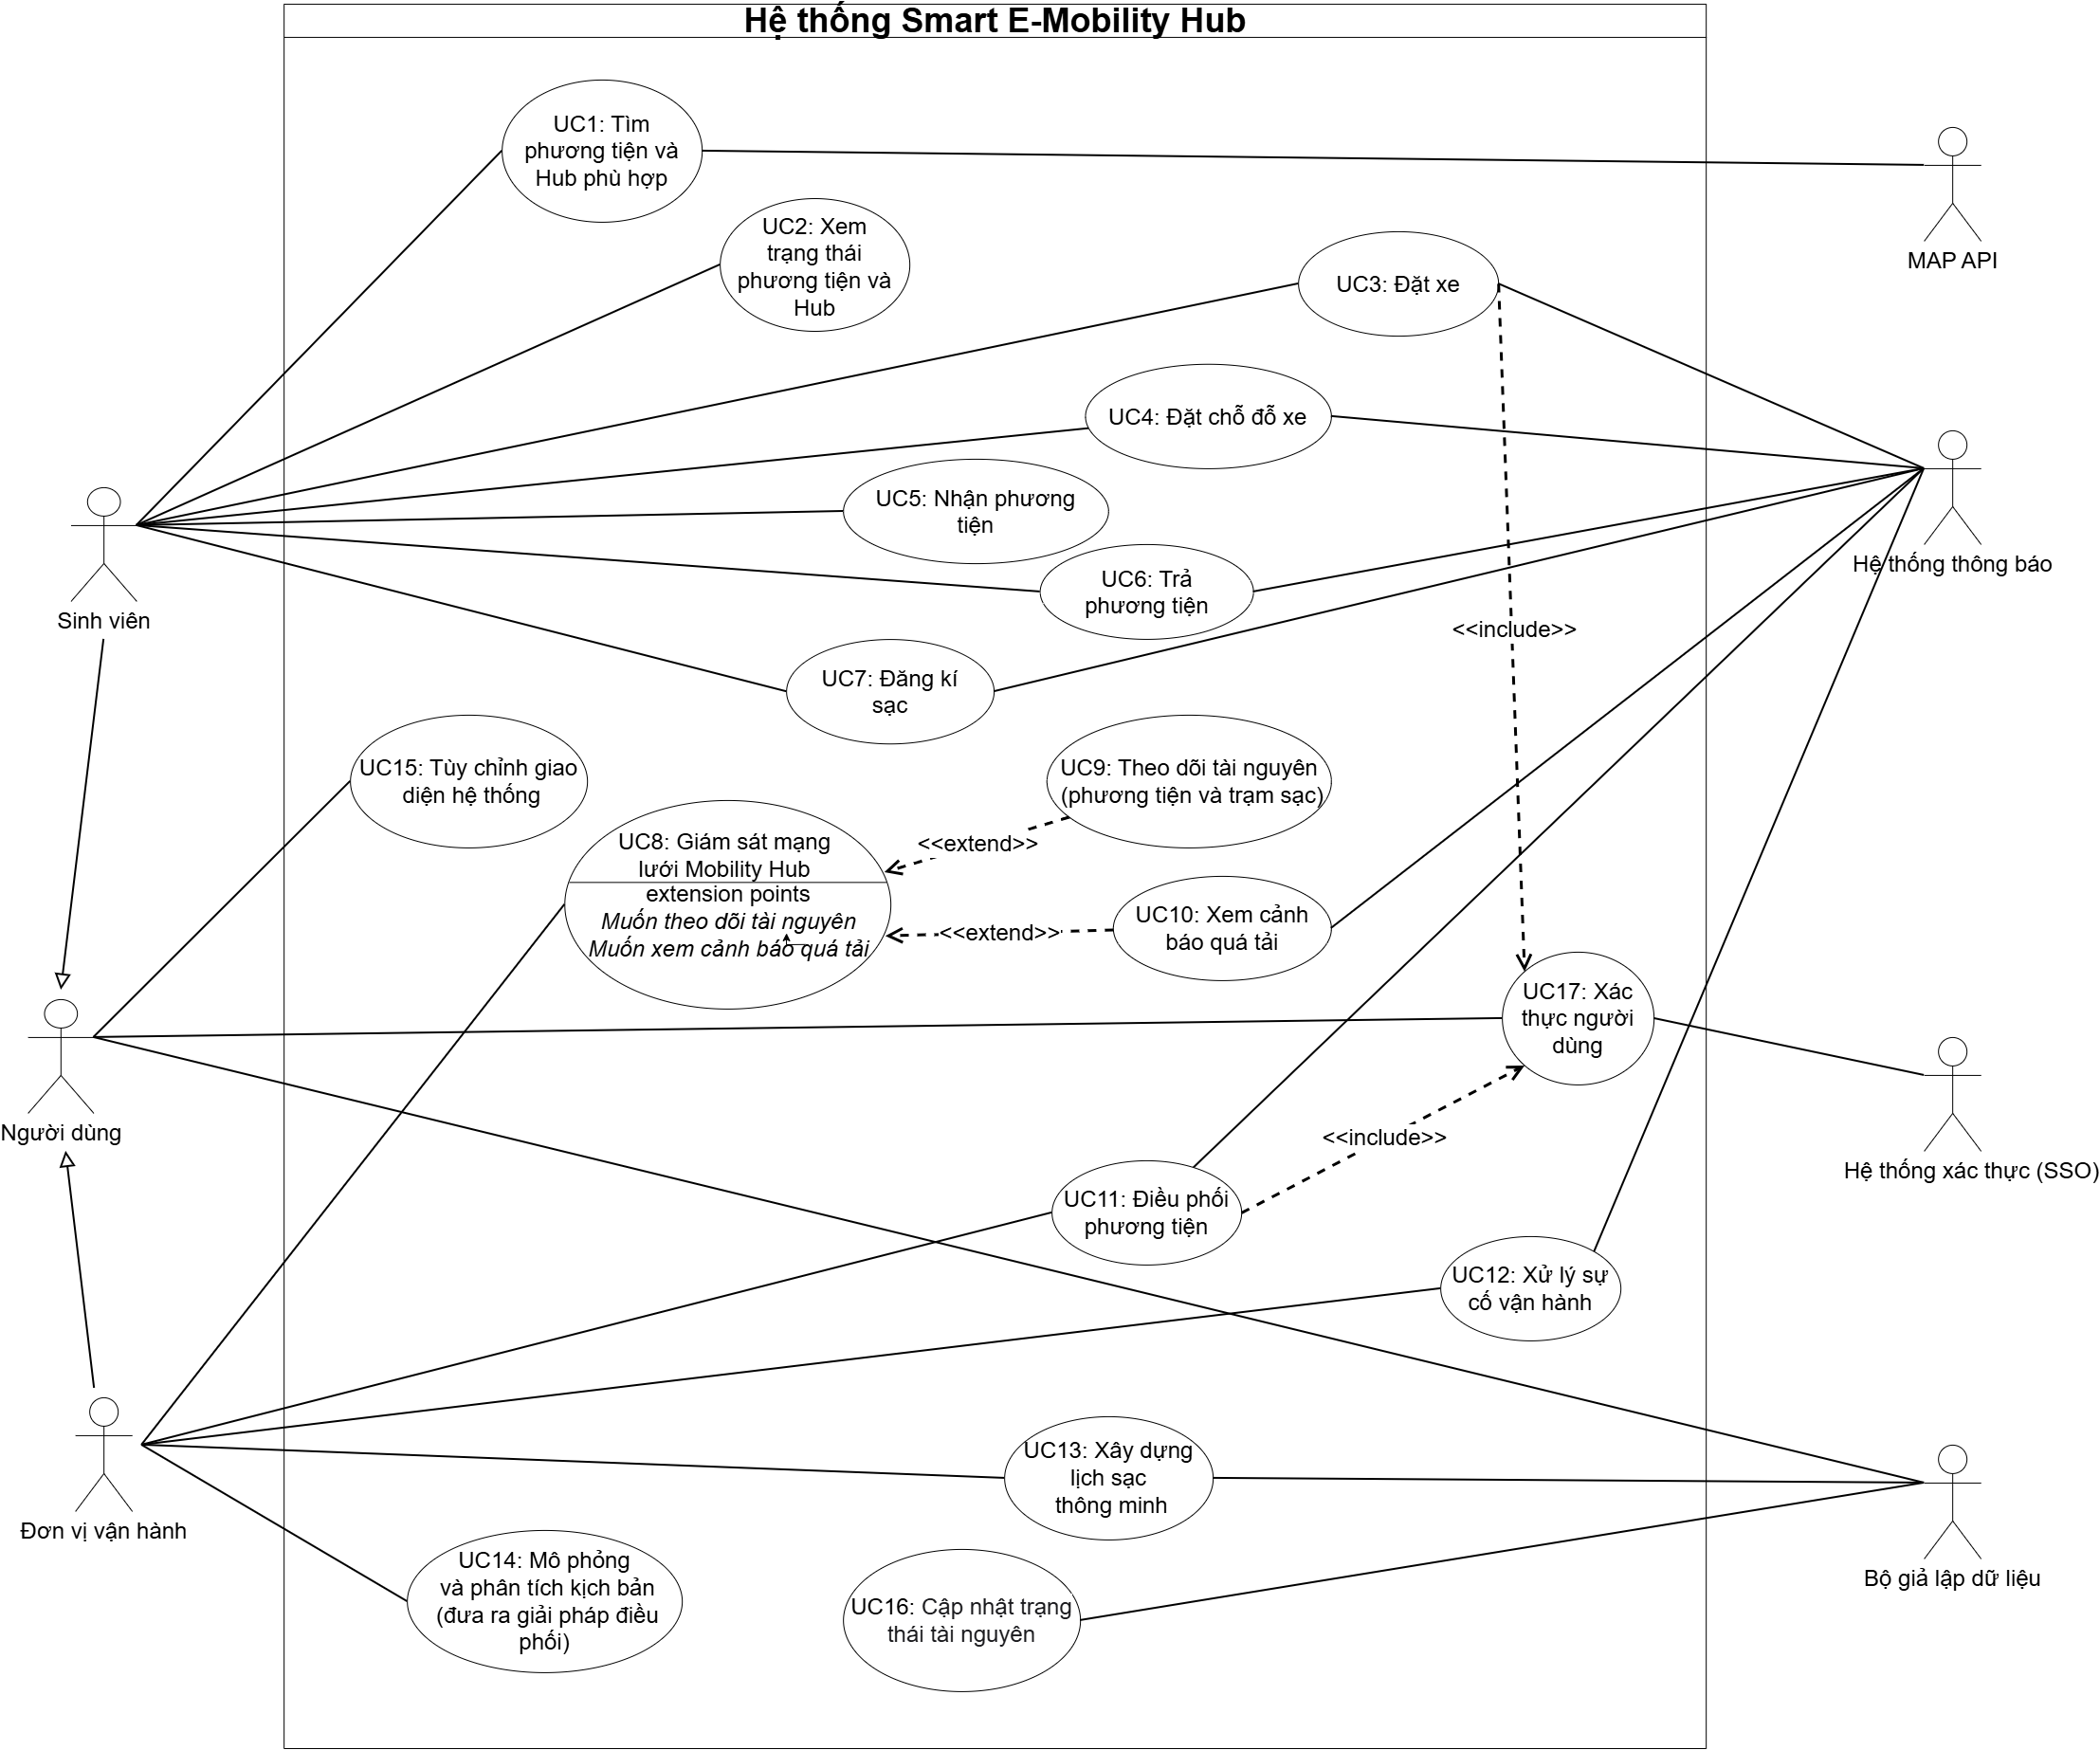
\includegraphics[width=0.98\textwidth,height=0.78\textheight,keepaspectratio]{s1/uc-diagram4.png}
\captionof{figure}{Sơ đồ Use Case của hệ thống Smart E-Mobility Hub}
\label{fig:usecase-diagram}
\end{center}
\noindent\textit{Ghi chú:} Actor Người dùng trên sơ đồ đóng vai trò là một Actor trừu tượng (\textit{Abstract Actor}), dùng để khái quát hóa quyền truy cập của cả Sinh viên và Đơn vị vận hành đối với các Use Case dùng chung.
\clearpage

\section{Đặc tả kịch bản Use Case (Use-case Scenarios)}

% Các bảng đặc tả được chuyển từ BBH BTL CNPM.pdf.

\subsection{Nhóm Use Case dành cho Sinh viên}

\subsubsection{UC1: Tìm phương tiện và Hub phù hợp}

{

\small

\setlength{\tabcolsep}{1pt}

\renewcommand{\arraystretch}{1.22}

\begin{longtable}{|>{\raggedright\arraybackslash}p{3.0cm}|>{\raggedright\arraybackslash}p{3.6cm}|>{\raggedright\arraybackslash}p{3.0cm}|>{\raggedright\arraybackslash}p{3.6cm}|}

\hline

\textbf{Field} & \multicolumn{3}{>{\raggedright\arraybackslash}p{10.2cm}|}{\textbf{Description}} \\

\hline

\endfirsthead

\hline

\textbf{Field} & \multicolumn{3}{>{\raggedright\arraybackslash}p{10.2cm}|}{\textbf{Description (tiếp theo)}} \\

\hline

\endhead

Use Case ID: & \multicolumn{3}{>{\raggedright\arraybackslash}p{10.2cm}|}{UC1} \\
\hline

Tên Use Case: & \multicolumn{3}{>{\raggedright\arraybackslash}p{10.2cm}|}{Tìm phương tiện và Hub phù hợp} \\
\hline

Tạo bởi: & Hoàng Phạm Tiến Thành & Lần cập nhật cuối bởi: & Hoàng Phạm Tiến Thành \\
\hline

Tạo vào ngày: & 18/09/2026 & Lần cập nhật cuối: & 19/09/2026 \\
\hline

Actors: & \multicolumn{3}{>{\raggedright\arraybackslash}p{10.2cm}|}{Sinh viên, Map API} \\
\hline

Mô tả: & \multicolumn{3}{>{\raggedright\arraybackslash}p{10.2cm}|}{Giúp sinh viên xác định các phương tiện điện dùng chung hoặc Mobility Hub phù hợp với vị trí và tiêu chí tìm kiếm, làm cơ sở để xem chi tiết hoặc thực hiện đặt tài nguyên.} \\
\hline

Trigger: & \multicolumn{3}{>{\raggedright\arraybackslash}p{10.2cm}|}{Sinh viên chọn chức năng “Tìm phương tiện và Hub”.} \\
\hline

Preconditions: & \multicolumn{3}{>{\raggedright\arraybackslash}p{10.2cm}|}{1. Sinh viên có thể truy cập giao diện tìm kiếm của hệ thống.\newline
2. Thông tin danh mục và tọa độ các Hub thuộc phạm vi phục vụ đã được cấu hình.\newline
3. Không bắt buộc sinh viên đăng nhập để thực hiện UC1.} \\
\hline

Postconditions: & \multicolumn{3}{>{\raggedright\arraybackslash}p{10.2cm}|}{1. Hệ thống hiển thị kết quả phù hợp với vị trí và tiêu chí đã chọn; hoặc thông báo không có kết quả phù hợp.\newline
2. Mỗi kết quả có thông tin tóm tắt và thời điểm cập nhật trạng thái để sinh viên đánh giá.\newline
3. Tiêu chí tìm kiếm được giữ trên giao diện để sinh viên điều chỉnh hoặc xem chi tiết kết quả.} \\
\hline

Normal Flow: & \multicolumn{3}{>{\raggedright\arraybackslash}p{10.2cm}|}{1. Sinh viên mở chức năng “Tìm phương tiện và Hub”.\newline
2. Hệ thống hiển thị giao diện tìm kiếm và bản đồ.\newline
3. Sinh viên chọn tìm phương tiện, sử dụng vị trí hiện tại và cấp quyền truy cập vị trí khi được yêu cầu.\newline
4. Hệ thống xác định và hiển thị vị trí tìm kiếm.\newline
5. Sinh viên chọn phạm vi khoảng cách, loại phương tiện, mức pin tối thiểu và gửi yêu cầu tìm kiếm.\newline
6. Hệ thống kiểm tra tính hợp lệ của thông tin, tìm các phương tiện khả dụng đáp ứng tiêu chí và sắp xếp theo khoảng cách đến Hub.\newline
7. Hệ thống hiển thị danh sách kết quả và vị trí Hub trên bản đồ, kèm thông tin tóm tắt về phương tiện, mức pin, trạng thái, khoảng cách và thời điểm cập nhật.\newline
8. Sinh viên xem kết quả. Use case kết thúc.} \\
\hline

Alternative Flows: & \multicolumn{3}{>{\raggedright\arraybackslash}p{10.2cm}|}{AF1: Tại bước 3, nhánh 3a --- Chọn vị trí thủ công. Sinh viên không sử dụng vị trí hiện tại hoặc từ chối cấp quyền định vị. Hệ thống cho phép chọn vị trí, khu vực hoặc Hub trên bản đồ; sau đó tiếp tục từ bước 4.\newline
AF2: Tại bước 3, nhánh 3b --- Tìm Hub thay vì tìm phương tiện. Hệ thống tìm theo khoảng cách, số xe khả dụng, số chỗ đỗ trống và số cổng sạc khả dụng; sau đó hiển thị kết quả Hub phù hợp.\newline
AF3: Tại bước 6, nhánh 6a --- Không có kết quả phù hợp. Hệ thống giữ điều kiện tìm kiếm và cho phép Sinh viên điều chỉnh rồi quay lại bước 5.\newline
AF4: Tại bước 7, nhánh 7a --- Điều chỉnh bộ lọc. Sinh viên thay đổi vị trí hoặc bộ lọc; hệ thống thực hiện lại từ bước 5.\newline
AF5: Tại bước 7, nhánh 7b --- Hủy tìm kiếm. Sinh viên rời khỏi màn hình tìm kiếm. Use case kết thúc, không thay đổi trạng thái tài nguyên.} \\
\hline

Exceptions: & \multicolumn{3}{>{\raggedright\arraybackslash}p{10.2cm}|}{EX1: Tại bước 3 --- Không xác định được vị trí. Thiết bị không cung cấp được tọa độ. Hệ thống thông báo lỗi và cho phép Sinh viên thử lại hoặc chuyển sang nhánh 3a.\newline
EX2: Tại bước 5 --- Tiêu chí tìm kiếm không hợp lệ. Hệ thống chỉ rõ thông tin cần chỉnh sửa và yêu cầu Sinh viên nhập lại trước khi quay lại bước 5.\newline
EX3: Tại bước 2 hoặc bước 7 --- Map API không khả dụng. Hệ thống thông báo lỗi bản đồ và chuyển sang hiển thị danh sách Hub theo khu vực hoặc tọa độ đã lưu.\newline
EX4: Tại bước 6 --- Không truy xuất được dữ liệu phương tiện/Hub hoặc mất kết nối. Hệ thống thông báo lỗi, giữ lại tiêu chí đã nhập và cho phép Sinh viên thử lại.} \\
\hline

FR liên quan: & \multicolumn{3}{>{\raggedright\arraybackslash}p{10.2cm}|}{FR01, FR13} \\
\hline
NFR liên quan: & \multicolumn{3}{>{\raggedright\arraybackslash}p{10.2cm}|}{NFR01, NFR02} \\
\hline
\end{longtable}

}

\clearpage

\subsubsection{UC2: Xem trạng thái phương tiện và Hub}

{

\small

\setlength{\tabcolsep}{1pt}

\renewcommand{\arraystretch}{1.22}

\begin{longtable}{|>{\raggedright\arraybackslash}p{3.0cm}|>{\raggedright\arraybackslash}p{3.6cm}|>{\raggedright\arraybackslash}p{3.0cm}|>{\raggedright\arraybackslash}p{3.6cm}|}

\hline

\textbf{Field} & \multicolumn{3}{>{\raggedright\arraybackslash}p{10.2cm}|}{\textbf{Description}} \\

\hline

\endfirsthead

\hline

\textbf{Field} & \multicolumn{3}{>{\raggedright\arraybackslash}p{10.2cm}|}{\textbf{Description (tiếp theo)}} \\

\hline

\endhead

Use Case ID: & \multicolumn{3}{>{\raggedright\arraybackslash}p{10.2cm}|}{UC2} \\
\hline

Tên Use Case: & \multicolumn{3}{>{\raggedright\arraybackslash}p{10.2cm}|}{Xem trạng thái phương tiện và Hub} \\
\hline

Tạo bởi: & Hoàng Phạm Tiến Thành & Lần cập nhật cuối bởi: & Hoàng Phạm Tiến Thành \\
\hline

Tạo vào ngày: & 18/09/2026 & Lần cập nhật cuối: & 19/09/2026 \\
\hline

Actors: & \multicolumn{3}{>{\raggedright\arraybackslash}p{10.2cm}|}{Sinh viên} \\
\hline

Mô tả: & \multicolumn{3}{>{\raggedright\arraybackslash}p{10.2cm}|}{Giúp Sinh viên xem trạng thái gần thời gian thực của một phương tiện hoặc Mobility Hub đã chọn để quyết định có tiếp tục tìm kiếm, đặt xe, đặt chỗ hoặc đăng ký sạc hay không.} \\
\hline

Trigger: & \multicolumn{3}{>{\raggedright\arraybackslash}p{10.2cm}|}{Sinh viên chọn chức năng “Xem trạng thái phương tiện và Hub” hoặc chọn một phương tiện/Hub từ kết quả của UC1.} \\
\hline

Preconditions: & \multicolumn{3}{>{\raggedright\arraybackslash}p{10.2cm}|}{1. Sinh viên có thể truy cập giao diện hệ thống.\newline
2. Phương tiện hoặc Hub cần xem có mã định danh trong hệ thống.\newline
3. Hệ thống có dữ liệu trạng thái gần nhất của tài nguyên hoặc có thể truy xuất dữ liệu đó.} \\
\hline

Postconditions: & \multicolumn{3}{>{\raggedright\arraybackslash}p{10.2cm}|}{1. Thành công: Hệ thống hiển thị trạng thái và thời điểm cập nhật gần nhất của tài nguyên được chọn.\newline
2. Thất bại hoặc hủy: Không có trạng thái tài nguyên, đơn đặt hoặc dữ liệu nào bị thay đổi.} \\
\hline

Normal Flow: & \multicolumn{3}{>{\raggedright\arraybackslash}p{10.2cm}|}{1. Sinh viên mở chức năng “Xem trạng thái phương tiện và Hub” hoặc chọn một phương tiện/Hub từ danh sách kết quả.\newline
2. Hệ thống xác định loại tài nguyên được chọn và truy xuất trạng thái gần nhất cùng thời điểm cập nhật.\newline
3. Hệ thống hiển thị thông tin chi tiết. Với phương tiện: loại xe, trạng thái, mức pin và Hub hiện tại. Với Hub: số phương tiện khả dụng, số chỗ đỗ trống, số cổng sạc khả dụng, mức độ sử dụng và thời điểm cập nhật.\newline
4. Sinh viên xem thông tin trạng thái. Use case kết thúc.} \\
\hline

Alternative Flows: & \multicolumn{3}{>{\raggedright\arraybackslash}p{10.2cm}|}{AF1: Tại bước 1, nhánh 1a --- Chọn xem phương tiện. Hệ thống hiển thị loại xe, trạng thái, mức pin và Hub hiện tại theo bước 2 và bước 3.\newline
AF2: Tại bước 1, nhánh 1b --- Chọn xem Hub. Hệ thống hiển thị số phương tiện khả dụng, chỗ đỗ trống, cổng sạc khả dụng và mức độ sử dụng theo bước 2 và bước 3.\newline
AF3: Tại bước 3, nhánh 3a --- Làm mới thông tin. Hệ thống truy xuất lại trạng thái gần nhất và thực hiện lại từ bước 2.\newline
AF4: Tại bước 3, nhánh 3b --- Tài nguyên không khả dụng. Hệ thống vẫn hiển thị trạng thái hiện tại, thời điểm cập nhật và cho phép Sinh viên chọn tài nguyên khác.\newline
AF5: Tại bước 3, nhánh 3c --- Chọn tài nguyên khác. Hệ thống thực hiện lại từ bước 1.\newline
AF6: Tại bước 4, nhánh 4a --- Rời màn hình. Use case kết thúc mà không thay đổi dữ liệu.} \\
\hline

Exceptions: & \multicolumn{3}{>{\raggedright\arraybackslash}p{10.2cm}|}{EX1: Tại bước 1 --- Chưa chọn tài nguyên hợp lệ. Hệ thống yêu cầu Sinh viên chọn phương tiện hoặc Hub trước khi tiếp tục.\newline
EX2: Tại bước 2 --- Tài nguyên không còn tồn tại hoặc đã ngừng hoạt động. Hệ thống thông báo và đưa Sinh viên về danh sách tìm kiếm hoặc danh sách tài nguyên.\newline
EX3: Tại bước 2 --- Không truy xuất được dữ liệu trạng thái. Hệ thống thông báo lỗi, giữ lại tài nguyên đang chọn và cho phép Sinh viên thử lại.\newline
EX4: Tại bước 2 --- Dữ liệu quá cũ hoặc chưa xác định. Hệ thống hiển thị thời điểm cập nhật gần nhất, đánh dấu dữ liệu chưa đáng tin cậy và không khẳng định tài nguyên còn khả dụng.} \\
\hline

FR liên quan: & \multicolumn{3}{>{\raggedright\arraybackslash}p{10.2cm}|}{FR02} \\
\hline
NFR liên quan: & \multicolumn{3}{>{\raggedright\arraybackslash}p{10.2cm}|}{NFR02} \\
\hline
\end{longtable}

}

\clearpage

\subsubsection{UC3: Đặt xe}

{

\small

\setlength{\tabcolsep}{1pt}

\renewcommand{\arraystretch}{1.22}

\begin{longtable}{|>{\raggedright\arraybackslash}p{3.0cm}|>{\raggedright\arraybackslash}p{3.6cm}|>{\raggedright\arraybackslash}p{3.0cm}|>{\raggedright\arraybackslash}p{3.6cm}|}

\hline

\textbf{Field} & \multicolumn{3}{>{\raggedright\arraybackslash}p{10.2cm}|}{\textbf{Description}} \\

\hline

\endfirsthead

\hline

\textbf{Field} & \multicolumn{3}{>{\raggedright\arraybackslash}p{10.2cm}|}{\textbf{Description (tiếp theo)}} \\

\hline

\endhead

Use Case ID: & \multicolumn{3}{>{\raggedright\arraybackslash}p{10.2cm}|}{UC3} \\
\hline

Tên Use Case: & \multicolumn{3}{>{\raggedright\arraybackslash}p{10.2cm}|}{Đặt xe} \\
\hline

Tạo bởi: & Nguyễn Khang Kỳ & Lần cập nhật cuối bởi: & Nguyễn Khang Kỳ \\
\hline

Tạo vào ngày: & 18/09/2026 & Lần cập nhật cuối: & 19/09/2026 \\
\hline

Actors: & \multicolumn{3}{>{\raggedright\arraybackslash}p{10.2cm}|}{Sinh viên; Hệ thống SSO; Hệ thống thông báo.} \\
\hline

Mô tả: & \multicolumn{3}{>{\raggedright\arraybackslash}p{10.2cm}|}{Sinh viên đặt trước phương tiện điện dùng chung tại Mobility Hub để có xe phục vụ hành trình di chuyển.} \\
\hline

Trigger: & \multicolumn{3}{>{\raggedright\arraybackslash}p{10.2cm}|}{Sinh viên chọn chức năng “Đặt xe” đối với phương tiện mong muốn.} \\
\hline

Preconditions: & \multicolumn{3}{>{\raggedright\arraybackslash}p{10.2cm}|}{1. Sinh viên có tài khoản SSO được phép sử dụng dịch vụ.\newline
2. Phương tiện và Hub đã có thông tin trên hệ thống.\newline
3. Sinh viên đã chọn một phương tiện cụ thể từ kết quả của UC1/UC2.} \\
\hline

Postconditions: & \multicolumn{3}{>{\raggedright\arraybackslash}p{10.2cm}|}{1. Thông tin đặt xe được lưu và gắn với sinh viên.\newline
2. Phương tiện chuyển sang trạng thái “Đã đặt”.\newline
3. Sinh viên nhận được thông tin xác nhận đặt xe.\newline
4. Nếu thất bại, không tạo đơn đặt và xe không bị giữ ở trạng thái không chính xác.} \\
\hline

Normal Flow: & \multicolumn{3}{>{\raggedright\arraybackslash}p{10.2cm}|}{1. Sinh viên chọn phương tiện và yêu cầu đặt xe.\newline
2. Hệ thống kiểm tra phiên làm việc hợp lệ và quyền sử dụng dịch vụ hợp lệ.\newline
3. Hệ thống hiển thị thông tin xe, mức pin và Hub nhận xe.\newline
4. Sinh viên kiểm tra thông tin và xác nhận đặt xe.\newline
5. Hệ thống thực hiện giao dịch nguyên tử: kiểm tra khả dụng, tạo đơn đặt, chuyển xe sang “Đã đặt” và ghi log.\newline
6. Hệ thống xác nhận giao dịch hoàn tất.\newline
7. Hệ thống hiển thị kết quả và, khi cần gửi ngoài ứng dụng, chuyển yêu cầu xác nhận đến Hệ thống thông báo.} \\
\hline

Alternative Flows: & \multicolumn{3}{>{\raggedright\arraybackslash}p{10.2cm}|}{AF1: Chọn phương tiện khác tại bước 3.\newline
3a. Sinh viên quay lại danh sách và chọn xe khác.\newline
3b. Hệ thống hiển thị thông tin phương tiện mới. Tiếp tục bước 4 của luồng chính.\newline
AF2: Hủy thao tác trước khi xác nhận tại bước 4.\newline
4a. Sinh viên chọn hủy đặt xe.\newline
4b. Hệ thống bỏ lựa chọn chưa lưu, không giữ xe. Use case kết thúc; không tạo đặt xe mới.} \\
\hline

Exceptions: & \multicolumn{3}{>{\raggedright\arraybackslash}p{10.2cm}|}{EX1: EX1: Phiên làm việc không hợp lệ hoặc đã hết hạn tại bước 2.\newline
2a. Hệ thống phát hiện phiên đăng nhập không còn hiệu lực.\newline
2b. Hệ thống lưu tạm lựa chọn phương tiện của sinh viên và thông báo yêu cầu xác thực.\newline
2c. Hệ thống tự động chuyển hướng người dùng sang màn hình đăng nhập (UC17).\newline
2d. Nếu xác thực thành công, hệ thống điều hướng sinh viên quay lại tiếp tục từ bước 3 của luồng chính. Nếu xác thực thất bại hoặc người dùng hủy, hệ thống xóa dữ liệu chọn xe tạm thời. Use case kết thúc.\newline
EX2: Xe không còn khả dụng tại bước 5.\newline
5a. Hệ thống thông báo xe đã được đặt, đang sử dụng hoặc không thể phục vụ.\newline
5b. Hệ thống làm mới danh sách để sinh viên chọn xe khác. Quay lại bước 1 hoặc kết thúc nếu sinh viên không tiếp tục.\newline
EX3: Không lưu được đặt xe tại bước 6.\newline
6a. Hệ thống thông báo chưa hoàn tất đặt xe.\newline
6b. Hệ thống kiểm tra kết quả lưu trước khi cho thử lại để tránh đặt trùng. Không xác nhận thành công khi chưa lưu được đặt xe.} \\
\hline

FR liên quan: & \multicolumn{3}{>{\raggedright\arraybackslash}p{10.2cm}|}{FR03, FR14} \\
\hline
NFR liên quan: & \multicolumn{3}{>{\raggedright\arraybackslash}p{10.2cm}|}{NFR09, NFR10, NFR11, NFR12} \\
\hline

\end{longtable}

}

\clearpage

\subsubsection{UC4: Đặt chỗ đỗ xe}

{

\small

\setlength{\tabcolsep}{1pt}

\renewcommand{\arraystretch}{1.22}

\begin{longtable}{|>{\raggedright\arraybackslash}p{3.0cm}|>{\raggedright\arraybackslash}p{3.6cm}|>{\raggedright\arraybackslash}p{3.0cm}|>{\raggedright\arraybackslash}p{3.6cm}|}

\hline

\textbf{Field} & \multicolumn{3}{>{\raggedright\arraybackslash}p{10.2cm}|}{\textbf{Description}} \\

\hline

\endfirsthead

\hline

\textbf{Field} & \multicolumn{3}{>{\raggedright\arraybackslash}p{10.2cm}|}{\textbf{Description (tiếp theo)}} \\

\hline

\endhead

Use Case ID: & \multicolumn{3}{>{\raggedright\arraybackslash}p{10.2cm}|}{UC4} \\
\hline

Tên Use Case: & \multicolumn{3}{>{\raggedright\arraybackslash}p{10.2cm}|}{Đặt chỗ đỗ xe} \\
\hline

Tạo bởi: & Nguyễn Khang Kỳ & Lần cập nhật cuối bởi: & Nguyễn Khang Kỳ \\
\hline

Tạo vào ngày: & 18/09/2026 & Lần cập nhật cuối: & 19/09/2026 \\
\hline

Actors: & \multicolumn{3}{>{\raggedright\arraybackslash}p{10.2cm}|}{Sinh viên; Hệ thống thông báo.} \\
\hline

Mô tả: & \multicolumn{3}{>{\raggedright\arraybackslash}p{10.2cm}|}{Sinh viên sử dụng phương tiện điện cá nhân đặt trước chỗ đỗ tại Mobility Hub để có vị trí đỗ phù hợp khi đến nơi.} \\
\hline

Trigger: & \multicolumn{3}{>{\raggedright\arraybackslash}p{10.2cm}|}{Sinh viên chọn chức năng “Đặt chỗ đỗ xe”.} \\
\hline

Preconditions: & \multicolumn{3}{>{\raggedright\arraybackslash}p{10.2cm}|}{1. Sinh viên có phiên đăng nhập hợp lệ và có quyền đặt chỗ.\newline
2. Thông tin Hub và chỗ đỗ đã được cấu hình trên hệ thống.\newline
3. Phương tiện cá nhân hoặc nhu cầu đỗ cần thiết đã được xác định.} \\
\hline

Postconditions: & \multicolumn{3}{>{\raggedright\arraybackslash}p{10.2cm}|}{1. Thông tin đặt chỗ được lưu cho sinh viên.\newline
2. Chỗ đỗ được giữ trong khoảng thời gian đã chọn.\newline
3. Thông tin chỗ đỗ và kết quả đăng ký được cập nhật trên hệ thống.} \\
\hline

Normal Flow: & \multicolumn{3}{>{\raggedright\arraybackslash}p{10.2cm}|}{1. Sinh viên chọn chức năng “Đặt chỗ đỗ xe”.\newline
2. Hệ thống hiển thị các Hub và thông tin chỗ đỗ.\newline
3. Sinh viên chọn Hub, vị trí đỗ và khoảng thời gian cần sử dụng.\newline
4. Hệ thống kiểm tra dữ liệu thời gian và hiển thị thông tin để xác nhận.\newline
5. Sinh viên xác nhận đặt chỗ.\newline
6. Hệ thống thực hiện giao dịch nguyên tử: kiểm tra lại khả dụng, lưu đặt chỗ, giữ vị trí trong khoảng thời gian đã chọn và ghi log.\newline
7. Hệ thống hiển thị kết quả và, khi cần gửi ngoài ứng dụng, chuyển yêu cầu xác nhận đến Hệ thống thông báo.} \\
\hline

Alternative Flows: & \multicolumn{3}{>{\raggedright\arraybackslash}p{10.2cm}|}{AF1: Thay đổi lựa chọn tại bước 4.\newline
4a. Sinh viên chọn thay đổi Hub, chỗ đỗ hoặc thời gian.\newline
4b. Hệ thống hiển thị lại các lựa chọn phù hợp. Quay lại bước 3 của luồng chính.\newline
AF2: Hủy thao tác trước khi xác nhận tại bước 5.\newline
5a. Sinh viên chọn hủy yêu cầu.\newline
5b. Hệ thống không lưu đăng ký mới và không giữ chỗ đỗ. Use case kết thúc.} \\
\hline

Exceptions: & \multicolumn{3}{>{\raggedright\arraybackslash}p{10.2cm}|}{EX1: Không còn chỗ phù hợp tại bước 4 hoặc 6.\newline
4a. Hệ thống thông báo chỗ đã được đặt hoặc không còn khả dụng trong khoảng thời gian yêu cầu.\newline
4b. Sinh viên có thể chọn chỗ khác, đổi Hub hoặc thời gian. Quay lại bước 3; kết thúc nếu sinh viên không tiếp tục.\newline
EX2: Khoảng thời gian không hợp lệ tại bước 4.\newline
4a. Hệ thống thông báo thời gian không hợp lệ, chẳng hạn thời điểm kết thúc trước thời điểm bắt đầu.\newline
4b. Sinh viên nhập lại thời gian. Quay lại bước 3 của luồng chính.\newline
EX3: Không lưu được đăng ký tại bước 6.\newline
6a. Hệ thống thông báo chưa hoàn tất đặt chỗ.\newline
6b. Hệ thống kiểm tra kết quả lưu trước khi cho sinh viên thử lại. Không xác nhận giữ chỗ nếu đăng ký chưa được lưu.} \\
\hline

FR liên quan: & \multicolumn{3}{>{\raggedright\arraybackslash}p{10.2cm}|}{FR03, FR14} \\
\hline
NFR liên quan: & \multicolumn{3}{>{\raggedright\arraybackslash}p{10.2cm}|}{NFR09, NFR10, NFR11, NFR12} \\
\hline

\end{longtable}

}

\clearpage

\subsubsection{UC5: Nhận phương tiện}

{

\small

\setlength{\tabcolsep}{1pt}

\renewcommand{\arraystretch}{1.22}

\begin{longtable}{|>{\raggedright\arraybackslash}p{3.0cm}|>{\raggedright\arraybackslash}p{3.6cm}|>{\raggedright\arraybackslash}p{3.0cm}|>{\raggedright\arraybackslash}p{3.6cm}|}

\hline

\textbf{Field} & \multicolumn{3}{>{\raggedright\arraybackslash}p{10.2cm}|}{\textbf{Description}} \\

\hline

\endfirsthead

\hline

\textbf{Field} & \multicolumn{3}{>{\raggedright\arraybackslash}p{10.2cm}|}{\textbf{Description (tiếp theo)}} \\

\hline

\endhead

Use Case ID: & \multicolumn{3}{>{\raggedright\arraybackslash}p{10.2cm}|}{UC5} \\
\hline

Tên Use Case: & \multicolumn{3}{>{\raggedright\arraybackslash}p{10.2cm}|}{Nhận phương tiện} \\
\hline

Tạo bởi: & Nguyễn Khang Kỳ & Lần cập nhật cuối bởi: & Nguyễn Khang Kỳ \\
\hline

Tạo vào ngày: & 18/09/2026 & Lần cập nhật cuối: & 19/09/2026 \\
\hline

Actors: & \multicolumn{3}{>{\raggedright\arraybackslash}p{10.2cm}|}{Sinh viên.} \\
\hline

Mô tả: & \multicolumn{3}{>{\raggedright\arraybackslash}p{10.2cm}|}{Sinh viên nhận phương tiện điện dùng chung đã đặt tại Mobility Hub để bắt đầu chuyến đi.} \\
\hline

Trigger: & \multicolumn{3}{>{\raggedright\arraybackslash}p{10.2cm}|}{Sinh viên chọn chức năng “Nhận phương tiện” trong thông tin đặt xe.} \\
\hline

Preconditions: & \multicolumn{3}{>{\raggedright\arraybackslash}p{10.2cm}|}{1. Sinh viên đã đăng nhập vào hệ thống.\newline
2. Sinh viên đã có thông tin đặt xe từ UC3.} \\
\hline

Postconditions: & \multicolumn{3}{>{\raggedright\arraybackslash}p{10.2cm}|}{1. Hệ thống ghi nhận sinh viên đã nhận đúng phương tiện.\newline
2. Trạng thái phương tiện chuyển sang “Đang sử dụng”; đặt xe chuyển sang “Đã nhận”.\newline
3. Thời điểm nhận xe và người nhận được lưu trên hệ thống.} \\
\hline

Normal Flow: & \multicolumn{3}{>{\raggedright\arraybackslash}p{10.2cm}|}{1. Sinh viên mở thông tin đặt xe và chọn “Nhận phương tiện”.\newline
2. Hệ thống kiểm tra người đặt, hiệu lực đặt xe, Hub nhận và trạng thái phương tiện.\newline
3. Sinh viên xác nhận đã nhận phương tiện trên giao diện; hệ thống chỉ mô phỏng và ghi nhận thao tác nhận, không điều khiển khóa vật lý.\newline
4. Hệ thống cập nhật xe sang “Đang sử dụng”, đặt xe sang “Đã nhận”, lưu thời điểm nhận và ghi log.\newline
5. Sau khi cập nhật thành công, hệ thống hiển thị xác nhận hoàn tất.} \\
\hline

Alternative Flows: & \multicolumn{3}{>{\raggedright\arraybackslash}p{10.2cm}|}{AF1: Chọn lại thông tin đặt xe tại bước 2.\newline
2a. Sinh viên quay lại danh sách đặt xe của mình.\newline
2b. Sinh viên chọn đúng đặt xe muốn nhận. Tiếp tục bước 2 để kiểm tra.\newline
AF2: Hủy yêu cầu nhận trước khi xác nhận tại bước 3.\newline
3a. Sinh viên chọn không tiếp tục nhận xe.\newline
3b. Hệ thống dừng thao tác nhận; đặt xe hiện có không bị hủy. Use case kết thúc; xe chưa chuyển sang “Đang sử dụng”.} \\
\hline

Exceptions: & \multicolumn{3}{>{\raggedright\arraybackslash}p{10.2cm}|}{EX1: Đặt xe không hợp lệ tại bước 2.\newline
2a. Hệ thống thông báo đặt xe không tồn tại, không thuộc sinh viên hoặc không còn hiệu lực.\newline
2b. Hệ thống không cho phép nhận phương tiện. Use case kết thúc.\newline
EX2: Phương tiện không thể nhận tại bước 2 hoặc 3.\newline
2a. Hệ thống thông báo xe không khả dụng hoặc có sự cố theo dữ liệu mô phỏng.\newline
2b. Sinh viên được hướng dẫn liên hệ đơn vị vận hành. Use case kết thúc; không ghi nhận nhận xe thành công.\newline
EX3: Lỗi cập nhật trạng thái tại bước 5.\newline
5a. Hệ thống thông báo quá trình nhận xe chưa hoàn tất cập nhật.\newline
5b. Hệ thống giữ thông tin nhận đã ghi, không cho người khác đặt xe này và chuyển đơn vị vận hành kiểm tra. Chưa xác nhận hoàn tất cho đến khi cập nhật thành công.} \\
\hline

FR liên quan: & \multicolumn{3}{>{\raggedright\arraybackslash}p{10.2cm}|}{FR03} \\
\hline
NFR liên quan: & \multicolumn{3}{>{\raggedright\arraybackslash}p{10.2cm}|}{NFR10, NFR11, NFR12} \\
\hline

\end{longtable}

}

\clearpage

\subsubsection{UC6: Trả phương tiện}

{

\small

\setlength{\tabcolsep}{1pt}

\renewcommand{\arraystretch}{1.22}

\begin{longtable}{|>{\raggedright\arraybackslash}p{3.0cm}|>{\raggedright\arraybackslash}p{3.6cm}|>{\raggedright\arraybackslash}p{3.0cm}|>{\raggedright\arraybackslash}p{3.6cm}|}

\hline

\textbf{Field} & \multicolumn{3}{>{\raggedright\arraybackslash}p{10.2cm}|}{\textbf{Description}} \\

\hline

\endfirsthead

\hline

\textbf{Field} & \multicolumn{3}{>{\raggedright\arraybackslash}p{10.2cm}|}{\textbf{Description (tiếp theo)}} \\

\hline

\endhead

Use Case ID: & \multicolumn{3}{>{\raggedright\arraybackslash}p{10.2cm}|}{UC6} \\
\hline

Tên Use Case: & \multicolumn{3}{>{\raggedright\arraybackslash}p{10.2cm}|}{Trả phương tiện} \\
\hline

Tạo bởi: & Võ Tấn Phát & Lần cập nhật cuối bởi: & Võ Tấn Phát \\
\hline

Tạo vào ngày: & 18/09/2026 & Lần cập nhật cuối: & 19/09/2026 \\
\hline

Actors: & \multicolumn{3}{>{\raggedright\arraybackslash}p{10.2cm}|}{Sinh viên, Hệ thống thông báo} \\
\hline

Mô tả: & \multicolumn{3}{>{\raggedright\arraybackslash}p{10.2cm}|}{Sinh viên trả phương tiện về cho hệ thống Smart Mobility Hub. Hệ thống thông báo sẽ cho biết phương tiện đã được trả về và có thể được mượn cho những người dùng khác.} \\
\hline

Trigger: & \multicolumn{3}{>{\raggedright\arraybackslash}p{10.2cm}|}{Sinh viên đưa phương tiện về Smart Mobility Hub và thực hiện chức năng “Trả phương tiện”.} \\
\hline

Preconditions: & \multicolumn{3}{>{\raggedright\arraybackslash}p{10.2cm}|}{1. Sinh viên có phiên đăng nhập hợp lệ và là người đang sử dụng phương tiện.\newline
2. Phương tiện đang được mượn và chưa được trả về.\newline
3. Hub nhận có khả năng tiếp nhận hoặc Sinh viên có chỗ đỗ đã đặt.} \\
\hline

Postconditions: & \multicolumn{3}{>{\raggedright\arraybackslash}p{10.2cm}|}{1. Phương tiện được đưa về trạng thái có sẵn trên hệ thống.\newline
2. Lượt mượn của sinh viên kết thúc.\newline
3. Hệ thống thông báo phương tiện đã được trả về thành công.} \\
\hline

Normal Flow: & \multicolumn{3}{>{\raggedright\arraybackslash}p{10.2cm}|}{1. Sinh viên đưa phương tiện về trạm Mobility Hub.\newline
2. Sinh viên thực hiện chức năng “Trả phương tiện”.\newline
3. Hệ thống kiểm tra người sử dụng, thông tin phương tiện, lượt mượn và khả năng tiếp nhận tại Hub.\newline
4. Hệ thống thực hiện giao dịch trả xe, lưu thời điểm, người trả, phương tiện và Hub nhận vào audit log.\newline
5. Hệ thống kết thúc lượt mượn.\newline
6. Hệ thống cập nhật trạng thái xe sang “Có sẵn”, “Chờ sạc” hoặc “Bảo trì” tùy mức pin và trạng thái kỹ thuật.\newline
7. Sau khi giao dịch thành công, hệ thống hiển thị và, khi cần gửi ngoài ứng dụng, gửi xác nhận trả phương tiện.} \\
\hline

Alternative Flows: & \multicolumn{3}{>{\raggedright\arraybackslash}p{10.2cm}|}{Không có.} \\
\hline

Exceptions: & \multicolumn{3}{>{\raggedright\arraybackslash}p{10.2cm}|}{EX1: Hệ thống không nhận diện được phương tiện hoặc không phát hiện lượt mượn tại bước 3.\newline
3a. Hệ thống thông báo phương tiện không hợp lệ.\newline
3b. Hệ thống yêu cầu sinh viên kiểm tra lại phương tiện và liên hệ đơn vị vận hành để hỗ trợ.\newline
3c. Hệ thống hủy yêu cầu trả phương tiện. Use case kết thúc.\newline
EX2: Hệ thống gặp lỗi kết nối mạng tại bước 4.\newline
4a. Hệ thống thông báo lỗi ghi nhận việc trả phương tiện không thành công.\newline
4b. Hệ thống yêu cầu sinh viên thử lại sau ít phút. Use case kết thúc; không ghi nhận việc trả phương tiện.\newline
EX3: Không thể gửi thông báo trả phương tiện tại bước 7.\newline
7a. Hệ thống ghi nhận thành công việc trả phương tiện.\newline
7b. Hệ thống ghi nhận lỗi thông báo và xử lý lại. Use case kết thúc; việc ghi nhận trả phương tiện vẫn thành công.} \\
\hline

FR liên quan: & \multicolumn{3}{>{\raggedright\arraybackslash}p{10.2cm}|}{FR03, FR14} \\
\hline
NFR liên quan: & \multicolumn{3}{>{\raggedright\arraybackslash}p{10.2cm}|}{NFR10, NFR11, NFR12} \\
\hline
\end{longtable}

}

\clearpage

\subsubsection{UC7: Đăng ký sạc}

{

\small

\setlength{\tabcolsep}{1pt}

\renewcommand{\arraystretch}{1.22}

\begin{longtable}{|>{\raggedright\arraybackslash}p{3.0cm}|>{\raggedright\arraybackslash}p{3.6cm}|>{\raggedright\arraybackslash}p{3.0cm}|>{\raggedright\arraybackslash}p{3.6cm}|}

\hline

\textbf{Field} & \multicolumn{3}{>{\raggedright\arraybackslash}p{10.2cm}|}{\textbf{Description}} \\

\hline

\endfirsthead

\hline

\textbf{Field} & \multicolumn{3}{>{\raggedright\arraybackslash}p{10.2cm}|}{\textbf{Description (tiếp theo)}} \\

\hline

\endhead

Use Case ID: & \multicolumn{3}{>{\raggedright\arraybackslash}p{10.2cm}|}{UC7} \\
\hline

Tên Use Case: & \multicolumn{3}{>{\raggedright\arraybackslash}p{10.2cm}|}{Đăng ký sạc} \\
\hline

Tạo bởi: & Võ Tấn Phát & Lần cập nhật cuối bởi: & Võ Tấn Phát \\
\hline

Tạo vào ngày: & 18/09/2026 & Lần cập nhật cuối: & 19/09/2026 \\
\hline

Actors: & \multicolumn{3}{>{\raggedright\arraybackslash}p{10.2cm}|}{Sinh viên; Hệ thống thông báo.} \\
\hline

Mô tả: & \multicolumn{3}{>{\raggedright\arraybackslash}p{10.2cm}|}{Sinh viên yêu cầu đăng ký lịch sạc cho phương tiện điện tại hệ thống Smart Mobility Hub.} \\
\hline

Trigger: & \multicolumn{3}{>{\raggedright\arraybackslash}p{10.2cm}|}{Sinh viên sử dụng chức năng “Đăng ký sạc”.} \\
\hline

Preconditions: & \multicolumn{3}{>{\raggedright\arraybackslash}p{10.2cm}|}{1. Sinh viên có phiên đăng nhập hợp lệ.\newline
2. Phương tiện cần sạc đã được khai báo hoặc đang thuộc lượt sử dụng hợp lệ của Sinh viên.\newline
3. Dữ liệu cổng sạc và khung giờ đã được cập nhật trong hệ thống.} \\
\hline

Postconditions: & \multicolumn{3}{>{\raggedright\arraybackslash}p{10.2cm}|}{1. Yêu cầu đăng ký sạc được lưu vào hệ thống.\newline
2. Vị trí sạc được đăng ký cho sinh viên theo thời gian đã chọn.\newline
3. Thông tin đăng ký sạc được cập nhật trên hệ thống.} \\
\hline

Normal Flow: & \multicolumn{3}{>{\raggedright\arraybackslash}p{10.2cm}|}{1. Sinh viên chọn chức năng “Đăng ký sạc”.\newline
2. Hệ thống hiển thị thông tin đăng ký sạc.\newline
3. Sinh viên xác nhận nhu cầu sạc.\newline
4. Hệ thống hiển thị các cổng sạc và mốc thời gian khả dụng.\newline
5. Sinh viên chọn cổng sạc và thời gian sạc.\newline
6. Hệ thống hiển thị lịch sạc để Sinh viên xác nhận.\newline
7. Sinh viên xác nhận đăng ký sạc.\newline
8. Hệ thống thực hiện giao dịch nguyên tử: kiểm tra lại khung giờ, tạo đăng ký, giữ cổng sạc và ghi audit log.\newline
9. Sau khi giao dịch hoàn tất, hệ thống hiển thị xác nhận và chuyển yêu cầu đến Hệ thống thông báo.} \\
\hline

Alternative Flows: & \multicolumn{3}{>{\raggedright\arraybackslash}p{10.2cm}|}{AF1: Tại bước 5 --- Sinh viên thay đổi cổng sạc hoặc thời gian. Hệ thống hiển thị lại các lựa chọn khả dụng; Sinh viên chọn lại và tiếp tục từ bước 6.\newline
AF2: Tại bước 6 --- Sinh viên hủy yêu cầu trước khi xác nhận. Hệ thống không lưu đăng ký hoặc giữ cổng sạc. Use case kết thúc.\newline
AF3: Tại bước 1 --- Sinh viên yêu cầu sạc khẩn cấp cho phương tiện đang sử dụng. Hệ thống lấy vị trí hiện tại, đề xuất Hub gần nhất có cổng sạc; sau khi Sinh viên xác nhận, hệ thống giữ cổng sạc và gửi xác nhận. Use case kết thúc.} \\
\hline

Exceptions: & \multicolumn{3}{>{\raggedright\arraybackslash}p{10.2cm}|}{EX1: Tại bước 4 --- Không còn cổng sạc hoặc khung giờ khả dụng. Hệ thống thông báo và cho phép Sinh viên thử lại sau.\newline
EX2: Tại bước 8 --- Khung giờ vừa được người khác đặt. Hệ thống trả về xung đột, không tạo đăng ký trùng và gợi ý cổng sạc, khung giờ hoặc Hub khác.\newline
EX3: Tại bước 8 --- Không thể lưu đăng ký. Hệ thống hủy các thay đổi tạm thời, ghi log lỗi và không xác nhận thành công.} \\
\hline

FR liên quan: & \multicolumn{3}{>{\raggedright\arraybackslash}p{10.2cm}|}{FR04, FR14} \\
\hline
NFR liên quan: & \multicolumn{3}{>{\raggedright\arraybackslash}p{10.2cm}|}{NFR09, NFR10, NFR11, NFR12} \\
\hline
\end{longtable}

}

\clearpage

\subsection{Nhóm Use Case dành cho Đơn vị vận hành}

\subsubsection{UC8: Giám sát mạng lưới Mobility Hub (Base Use Case)}

{

\small

\setlength{\tabcolsep}{1pt}

\renewcommand{\arraystretch}{1.22}

\begin{longtable}{|>{\raggedright\arraybackslash}p{3.0cm}|>{\raggedright\arraybackslash}p{3.6cm}|>{\raggedright\arraybackslash}p{3.0cm}|>{\raggedright\arraybackslash}p{3.6cm}|}

\hline

\textbf{Field} & \multicolumn{3}{>{\raggedright\arraybackslash}p{10.2cm}|}{\textbf{Description}} \\

\hline

\endfirsthead

\hline

\textbf{Field} & \multicolumn{3}{>{\raggedright\arraybackslash}p{10.2cm}|}{\textbf{Description (tiếp theo)}} \\

\hline

\endhead

Use Case ID: & \multicolumn{3}{>{\raggedright\arraybackslash}p{10.2cm}|}{UC8} \\
\hline

Tên Use Case: & \multicolumn{3}{>{\raggedright\arraybackslash}p{10.2cm}|}{Giám sát mạng lưới Mobility Hub} \\
\hline

Tạo bởi: & Hoàng Phạm Tiến Thành & Lần cập nhật cuối bởi: & Hoàng Phạm Tiến Thành \\
\hline

Tạo vào ngày: & 18/09/2026 & Lần cập nhật cuối: & 19/09/2026 \\
\hline

Actors: & \multicolumn{3}{>{\raggedright\arraybackslash}p{10.2cm}|}{Đơn vị vận hành} \\
\hline

Mô tả: & \multicolumn{3}{>{\raggedright\arraybackslash}p{10.2cm}|}{Cung cấp cho Đơn vị vận hành cái nhìn tổng quan, gần thời gian thực về tình trạng của toàn bộ mạng lưới Mobility Hub để đánh giá mức độ sử dụng và quyết định có cần theo dõi chi tiết, xem cảnh báo hoặc thực hiện các hoạt động điều phối hay không.} \\
\hline

Trigger: & \multicolumn{3}{>{\raggedright\arraybackslash}p{10.2cm}|}{Đơn vị vận hành chọn chức năng “Giám sát mạng lưới Mobility Hub” trên hệ thống.} \\
\hline

Preconditions: & \multicolumn{3}{>{\raggedright\arraybackslash}p{10.2cm}|}{1. Người dùng đã được xác thực qua SSO và có quyền Đơn vị vận hành.\newline
2. Thông tin các Mobility Hub đã được cấu hình trong hệ thống.\newline
3. Hệ thống có dữ liệu trạng thái gần nhất của mạng lưới hoặc có thể truy xuất dữ liệu đó.} \\
\hline

Postconditions: & \multicolumn{3}{>{\raggedright\arraybackslash}p{10.2cm}|}{1. Thành công: Hệ thống hiển thị dashboard tổng quan về trạng thái mạng lưới và thời điểm cập nhật gần nhất của dữ liệu.\newline
2. Thất bại hoặc hủy: Không có trạng thái tài nguyên hoặc dữ liệu vận hành nào bị thay đổi.} \\
\hline

Normal Flow: & \multicolumn{3}{>{\raggedright\arraybackslash}p{10.2cm}|}{1. Đơn vị vận hành mở chức năng “Giám sát mạng lưới Mobility Hub”.\newline
2. Hệ thống kiểm tra phiên làm việc và quyền truy cập của người dùng.\newline
3. Hệ thống truy xuất dữ liệu trạng thái gần nhất của các Hub, phương tiện, chỗ đỗ và cổng sạc trong mạng lưới.\newline
4. Hệ thống tổng hợp mức độ sử dụng và trạng thái hoạt động của từng Hub.\newline
5. Hệ thống hiển thị dashboard tổng quan, bao gồm số lượng Hub đang hoạt động, số phương tiện khả dụng, số chỗ đỗ trống, số cổng sạc khả dụng, mức độ sử dụng của từng Hub và thời điểm cập nhật gần nhất.\newline
6. Đơn vị vận hành xem thông tin tổng quan. Use case kết thúc.} \\
\hline

Alternative Flows: & \multicolumn{3}{>{\raggedright\arraybackslash}p{10.2cm}|}{AF1: Tại bước 5 $\rightarrow$ 5a --- Lọc thông tin giám sát. Đơn vị vận hành lọc các Hub theo khu vực, trạng thái hoạt động hoặc mức độ sử dụng. Hệ thống cập nhật dashboard theo tiêu chí đã chọn và quay lại bước 5.\newline
AF2: Tại bước 5 $\rightarrow$ 5b --- Làm mới dashboard. Đơn vị vận hành yêu cầu làm mới. Hệ thống truy xuất dữ liệu gần nhất, sau đó thực hiện lại từ bước 3.\newline
AF3: Tại bước 5 $\rightarrow$ 5c --- Theo dõi chi tiết tài nguyên. Đơn vị vận hành chọn một Hub hoặc nhóm tài nguyên cần xem sâu hơn. Hệ thống thực hiện UC9 “Theo dõi tài nguyên”; khi kết thúc UC9, hệ thống quay lại bước 5 của UC8.\newline
AF4: Tại bước 5 $\rightarrow$ 5d --- Xem cảnh báo quá tải. Đơn vị vận hành chọn xem cảnh báo liên quan đến Hub có nguy cơ quá tải. Hệ thống thực hiện UC10 “Xem cảnh báo quá tải”; khi kết thúc UC10, hệ thống quay lại bước 5 của UC8.\newline
AF5: Tại bước 5a $\rightarrow$ 5a.1 --- Không có Hub phù hợp với bộ lọc. Hệ thống thông báo không có Hub đáp ứng tiêu chí, giữ nguyên bộ lọc để Đơn vị vận hành điều chỉnh hoặc xóa bộ lọc.} \\
\hline

Exceptions: & \multicolumn{3}{>{\raggedright\arraybackslash}p{10.2cm}|}{EX1: Tại bước 2 --- Phiên đăng nhập không hợp lệ hoặc không đủ quyền. Hệ thống từ chối truy cập và yêu cầu người dùng xác thực lại bằng tài khoản có quyền vận hành.\newline
EX2: Tại bước 3 --- Không truy xuất được dữ liệu giám sát. Hệ thống thông báo không thể tải dashboard và cho phép Đơn vị vận hành thử lại.\newline
EX3: Tại bước 3 $\rightarrow$ 3a --- Dữ liệu một phần hoặc quá cũ. Hệ thống hiển thị dữ liệu gần nhất có thể truy xuất, đánh dấu Hub/tài nguyên có dữ liệu chưa xác định cùng thời điểm cập nhật; không khẳng định các tài nguyên đó đang khả dụng.\newline
EX4: Tại bước 4 --- Dữ liệu cấu hình Hub không hợp lệ. Hệ thống đánh dấu Hub cần kiểm tra và không dùng dữ liệu thiếu sức chứa hoặc trạng thái để tính mức độ sử dụng.} \\
\hline

FR liên quan: & \multicolumn{3}{>{\raggedright\arraybackslash}p{10.2cm}|}{FR05} \\
\hline
NFR liên quan: & \multicolumn{3}{>{\raggedright\arraybackslash}p{10.2cm}|}{NFR02, NFR05, NFR10} \\
\hline
\end{longtable}

}

\clearpage

\subsubsection{UC9: Theo dõi tài nguyên (phương tiện và trạm sạc) (Extend UC8)}

{

\small

\setlength{\tabcolsep}{1pt}

\renewcommand{\arraystretch}{1.22}

\begin{longtable}{|>{\raggedright\arraybackslash}p{3.0cm}|>{\raggedright\arraybackslash}p{3.6cm}|>{\raggedright\arraybackslash}p{3.0cm}|>{\raggedright\arraybackslash}p{3.6cm}|}

\hline

\textbf{Field} & \multicolumn{3}{>{\raggedright\arraybackslash}p{10.2cm}|}{\textbf{Description}} \\

\hline

\endfirsthead

\hline

\textbf{Field} & \multicolumn{3}{>{\raggedright\arraybackslash}p{10.2cm}|}{\textbf{Description (tiếp theo)}} \\

\hline

\endhead

Use Case ID: & \multicolumn{3}{>{\raggedright\arraybackslash}p{10.2cm}|}{UC9} \\
\hline

Tên Use Case: & \multicolumn{3}{>{\raggedright\arraybackslash}p{10.2cm}|}{Theo dõi tài nguyên (phương tiện và trạm sạc)} \\
\hline

Tạo bởi: & Võ Tấn Phát & Lần cập nhật cuối bởi: & Võ Tấn Phát \\
\hline

Tạo vào ngày: & 18/09/2026 & Lần cập nhật cuối: & 19/09/2026 \\
\hline

Actors: & \multicolumn{3}{>{\raggedright\arraybackslash}p{10.2cm}|}{Đơn vị vận hành} \\
\hline

Mô tả: & \multicolumn{3}{>{\raggedright\arraybackslash}p{10.2cm}|}{Cho phép đơn vị vận hành kiểm tra thông tin của các phương tiện và trạm sạc trong hệ thống Smart Mobility Hub, bao gồm: tình trạng phương tiện, mức pin, vị trí đỗ, tình trạng cổng sạc và mức sử dụng của từng Hub.} \\
\hline

Trigger: & \multicolumn{3}{>{\raggedright\arraybackslash}p{10.2cm}|}{Trong quá trình thực hiện UC8: Giám sát mạng lưới Mobility Hub, đơn vị vận hành chọn chức năng “Theo dõi tài nguyên”.} \\
\hline

Preconditions: & \multicolumn{3}{>{\raggedright\arraybackslash}p{10.2cm}|}{1. UC8 đang được vận hành.\newline
2. Hệ thống có dữ liệu tài nguyên cần theo dõi.} \\
\hline

Postconditions: & \multicolumn{3}{>{\raggedright\arraybackslash}p{10.2cm}|}{1. Hệ thống hiển thị thông tin của tài nguyên cho đơn vị vận hành theo dõi.\newline
2. Đơn vị vận hành có thể tiếp tục giám sát mạng lưới Mobility Hub.} \\
\hline

Normal Flow: & \multicolumn{3}{>{\raggedright\arraybackslash}p{10.2cm}|}{1. Đơn vị vận hành đang thực hiện UC8 với phiên đăng nhập và quyền hợp lệ.\newline
2. Đơn vị vận hành thực hiện chức năng “Theo dõi tài nguyên”.\newline
3. Hệ thống truy xuất dữ liệu tài nguyên hiện tại cùng thời điểm cập nhật.\newline
4. Hệ thống hiển thị trạng thái, thời điểm cập nhật và đánh dấu dữ liệu quá cũ/chưa xác định khi cần.\newline
5. Đơn vị vận hành có thể quay về UC8 hoặc kết thúc việc theo dõi.} \\
\hline

Alternative Flows: & \multicolumn{3}{>{\raggedright\arraybackslash}p{10.2cm}|}{AF1: Lọc tài nguyên theo Hub, loại tài nguyên hoặc trạng thái. Hệ thống cập nhật danh sách theo tiêu chí đã chọn.\newline
AF2: Làm mới thông tin. Hệ thống truy xuất lại trạng thái gần nhất và tiếp tục từ bước 3.\newline
AF3: Chọn tài nguyên khác. Hệ thống thực hiện lại từ bước 3 cho tài nguyên được chọn.} \\
\hline

Exceptions: & \multicolumn{3}{>{\raggedright\arraybackslash}p{10.2cm}|}{EX1: Hệ thống không thể truy xuất dữ liệu tại bước 3.\newline
3a. Hệ thống thông báo lỗi truy cập dữ liệu.\newline
3b. Hệ thống yêu cầu Đơn vị vận hành thử lại.\newline
3c. Hệ thống hủy yêu cầu theo dõi dữ liệu.\newline
EX2: Dữ liệu tài nguyên không khả dụng tại bước 3.\newline
3a. Hệ thống thông báo tài nguyên chưa được cập nhật.\newline
3b. Hệ thống không hiển thị thông tin tài nguyên.\newline
3c. Hệ thống kết thúc yêu cầu.} \\
\hline

FR liên quan: & \multicolumn{3}{>{\raggedright\arraybackslash}p{10.2cm}|}{FR06} \\
\hline
NFR liên quan: & \multicolumn{3}{>{\raggedright\arraybackslash}p{10.2cm}|}{NFR02, NFR10} \\
\hline
\end{longtable}

}

\clearpage

\subsubsection{UC10: Xem cảnh báo quá tải (Extend UC8)}

{

\small

\setlength{\tabcolsep}{1pt}

\renewcommand{\arraystretch}{1.22}

\begin{longtable}{|>{\raggedright\arraybackslash}p{3.0cm}|>{\raggedright\arraybackslash}p{3.6cm}|>{\raggedright\arraybackslash}p{3.0cm}|>{\raggedright\arraybackslash}p{3.6cm}|}

\hline

\textbf{Field} & \multicolumn{3}{>{\raggedright\arraybackslash}p{10.2cm}|}{\textbf{Description}} \\

\hline

\endfirsthead

\hline

\textbf{Field} & \multicolumn{3}{>{\raggedright\arraybackslash}p{10.2cm}|}{\textbf{Description (tiếp theo)}} \\

\hline

\endhead

Use Case ID: & \multicolumn{3}{>{\raggedright\arraybackslash}p{10.2cm}|}{UC10} \\
\hline

Tên Use Case: & \multicolumn{3}{>{\raggedright\arraybackslash}p{10.2cm}|}{Xem cảnh báo quá tải} \\
\hline

Tạo bởi: & Võ Tấn Phát & Lần cập nhật cuối bởi: & Võ Tấn Phát \\
\hline

Tạo vào ngày: & 18/09/2026 & Lần cập nhật cuối: & 19/09/2026 \\
\hline

Actors: & \multicolumn{3}{>{\raggedright\arraybackslash}p{10.2cm}|}{Đơn vị vận hành; Hệ thống thông báo.} \\
\hline

Mô tả: & \multicolumn{3}{>{\raggedright\arraybackslash}p{10.2cm}|}{Cho phép Đơn vị vận hành xem các cảnh báo quá tải do Smart E-Mobility Hub tạo từ dữ liệu trạng thái mạng lưới. Hệ thống thông báo chỉ được dùng để phân phối cảnh báo ra ngoài ứng dụng khi cần.} \\
\hline

Trigger: & \multicolumn{3}{>{\raggedright\arraybackslash}p{10.2cm}|}{Đơn vị vận hành chọn chức năng “Xem cảnh báo quá tải” từ dashboard UC8 hoặc mở danh sách cảnh báo.} \\
\hline

Preconditions: & \multicolumn{3}{>{\raggedright\arraybackslash}p{10.2cm}|}{1. Đơn vị vận hành có phiên đăng nhập hợp lệ và đúng quyền.\newline
2. UC8 đang hoạt động hoặc người vận hành mở danh sách cảnh báo.} \\
\hline

Postconditions: & \multicolumn{3}{>{\raggedright\arraybackslash}p{10.2cm}|}{1. Hệ thống hiển thị cảnh báo hiện có hoặc trạng thái mạng lưới bình thường.\newline
2. Không có dữ liệu vận hành nào bị thay đổi.} \\
\hline

Normal Flow: & \multicolumn{3}{>{\raggedright\arraybackslash}p{10.2cm}|}{1. Đơn vị vận hành chọn xem cảnh báo quá tải từ dashboard.\newline
2. Hệ thống truy xuất các cảnh báo do Smart E-Mobility Hub tạo từ dữ liệu mạng lưới.\newline
3. Hệ thống hiển thị Hub liên quan, chỉ số sử dụng, mức độ cảnh báo và thời điểm phát hiện.\newline
4. Đơn vị vận hành chọn một cảnh báo để xem chi tiết.\newline
5. Hệ thống hiển thị nguyên nhân dự kiến và các hành động liên quan như UC11 hoặc UC13.} \\
\hline

Alternative Flows: & \multicolumn{3}{>{\raggedright\arraybackslash}p{10.2cm}|}{AF1: Tại bước 2 --- Không có cảnh báo. Hệ thống hiển thị trạng thái mạng lưới bình thường và quay lại UC8.} \\
\hline

Exceptions: & \multicolumn{3}{>{\raggedright\arraybackslash}p{10.2cm}|}{EX1: Tại bước 2 --- Không truy xuất được dữ liệu cảnh báo. Hệ thống thông báo lỗi và giữ nguyên dashboard để Đơn vị vận hành thử lại.} \\
\hline

FR liên quan: & \multicolumn{3}{>{\raggedright\arraybackslash}p{10.2cm}|}{FR06, FR14} \\
\hline
NFR liên quan: & \multicolumn{3}{>{\raggedright\arraybackslash}p{10.2cm}|}{NFR02, NFR10} \\
\hline
\end{longtable}

}

\clearpage

\subsubsection{UC11: Điều phối phương tiện}

{

\small

\setlength{\tabcolsep}{1pt}

\renewcommand{\arraystretch}{1.22}

\begin{longtable}{|>{\raggedright\arraybackslash}p{3.0cm}|>{\raggedright\arraybackslash}p{3.6cm}|>{\raggedright\arraybackslash}p{3.0cm}|>{\raggedright\arraybackslash}p{3.6cm}|}

\hline

\textbf{Field} & \multicolumn{3}{>{\raggedright\arraybackslash}p{10.2cm}|}{\textbf{Description}} \\

\hline

\endfirsthead

\hline

\textbf{Field} & \multicolumn{3}{>{\raggedright\arraybackslash}p{10.2cm}|}{\textbf{Description (tiếp theo)}} \\

\hline

\endhead

Use Case ID: & \multicolumn{3}{>{\raggedright\arraybackslash}p{10.2cm}|}{UC11} \\
\hline

Tên Use Case: & \multicolumn{3}{>{\raggedright\arraybackslash}p{10.2cm}|}{Điều phối phương tiện} \\
\hline

Tạo bởi: & Đào Huy Phong & Lần cập nhật cuối bởi: & Đào Huy Phong \\
\hline

Tạo vào ngày: & 18/09/2026 & Lần cập nhật cuối: & 19/09/2026 \\
\hline

Actors: & \multicolumn{3}{>{\raggedright\arraybackslash}p{10.2cm}|}{Đơn vị vận hành, Hệ thống thông báo} \\
\hline

Mô tả: & \multicolumn{3}{>{\raggedright\arraybackslash}p{10.2cm}|}{Cho phép Đơn vị vận hành lập lệnh và thực hiện di chuyển phương tiện dùng chung từ Hub đang dư xe đến Hub đang thiếu xe hoặc có nhu cầu tăng cao, giúp cân bằng tài nguyên trong mạng lưới.} \\
\hline

Trigger: & \multicolumn{3}{>{\raggedright\arraybackslash}p{10.2cm}|}{Đơn vị vận hành chọn chức năng “Điều phối phương tiện” từ giao diện quản trị hoặc sau khi nhận được cảnh báo mất cân bằng / quá tải (UC10).} \\
\hline

Preconditions: & \multicolumn{3}{>{\raggedright\arraybackslash}p{10.2cm}|}{1. Người dùng đã được xác thực qua SSO với vai trò Đơn vị vận hành (NFR10).\newline
2. Hệ thống có dữ liệu trạng thái thời gian thực của các Hub và phương tiện (NFR02).} \\
\hline

Postconditions: & \multicolumn{3}{>{\raggedright\arraybackslash}p{10.2cm}|}{1. Lệnh điều phối được tạo thành công, ghi nhận danh sách xe, Hub xuất phát và Hub đích.\newline
2. Trạng thái các xe liên quan chuyển sang “Đang điều phối” (không cho phép Sinh viên đặt - NFR09).\newline
3. Mọi thao tác và thay đổi trạng thái được ghi log lịch sử hệ thống (NFR11).\newline
4. Thông báo được gửi đến đội ngũ nhân sự vận chuyển thực địa.} \\
\hline

Normal Flow: & \multicolumn{3}{>{\raggedright\arraybackslash}p{10.2cm}|}{1. Đơn vị vận hành mở chức năng Điều phối phương tiện.\newline
2. Hệ thống kiểm tra quyền truy cập và hiển thị bản đồ/bảng cân bằng phương tiện tại các Hub.\newline
3. Đơn vị vận hành chọn Hub nguồn và Hub đích.\newline
4. Hệ thống hiển thị phương tiện khả dụng tại Hub nguồn kèm mức pin.\newline
5. Hệ thống kiểm tra Hub đích đủ chỗ đỗ cho số xe dự kiến điều phối.\newline
6. Đơn vị vận hành chọn danh sách xe và xác nhận lệnh.\newline
7. Hệ thống thực hiện giao dịch nguyên tử: khóa xe, tạo lệnh, đổi trạng thái xe sang “Đang điều phối”, cập nhật sức chứa dự kiến và ghi log.\newline
8. Hệ thống chuyển yêu cầu thông báo công việc đến Hệ thống thông báo.\newline
9. Hệ thống hiển thị tạo lệnh điều phối thành công. Use case kết thúc.} \\
\hline

Alternative Flows: & \multicolumn{3}{>{\raggedright\arraybackslash}p{10.2cm}|}{AF1: Tại bước 3 $\rightarrow$ 3a --- Áp dụng phương án từ UC14. Đơn vị vận hành chọn áp dụng một phương án điều phối do UC14 gợi ý.\newline
3b. Hệ thống tự động điền Hub nguồn, Hub đích và danh sách phương tiện được đề xuất.\newline
3c. Đơn vị vận hành kiểm tra, điều chỉnh nếu cần và tiếp tục từ bước 5.\newline
AF2: Tại bước 7 $\rightarrow$ 7a --- Hủy lệnh điều phối khi chưa vận chuyển. Đơn vị vận hành chọn một lệnh đang ở trạng thái chờ xử lý và yêu cầu hủy.\newline
7b. Hệ thống mở khóa các phương tiện liên quan, khôi phục trạng thái “Khả dụng” tại Hub nguồn và cập nhật lại sức chứa dự kiến của các Hub.\newline
7c. Hệ thống lưu log, gửi thông báo liên quan và kết thúc use case.} \\
\hline

Exceptions: & \multicolumn{3}{>{\raggedright\arraybackslash}p{10.2cm}|}{EX1: Phiên đăng nhập hoặc quyền truy cập không hợp lệ tại bước 2.\newline
2a. Hệ thống phát hiện phiên làm việc đã hết hạn hoặc tài khoản hiện tại không có vai trò Đơn vị vận hành.\newline
2b. Hệ thống chặn truy cập, từ chối tải dữ liệu bản đồ và hiển thị cảnh báo lỗi "Không đủ quyền truy cập hoặc phiên làm việc đã hết hạn".\newline
2c. Hệ thống yêu cầu người dùng xác thực lại và điều hướng sang màn hình đăng nhập (UC17). Use case kết thúc.\newline
EX2: Tại bước 5 --- Hub đích không đủ chỗ đỗ. Hệ thống thông báo Hub đích không đủ sức chứa, yêu cầu Đơn vị vận hành giảm số xe điều phối hoặc chọn Hub đích khác; quay lại bước 3 hoặc bước 5.\newline
EX3: Tại bước 6 --- Không tạo được lệnh điều phối. Hệ thống không thể hoàn tất giao dịch hoặc cập nhật trạng thái xe. Hệ thống hủy các thay đổi tạm thời, ghi log lỗi và cho phép Đơn vị vận hành thử lại.} \\
\hline

FR liên quan: & \multicolumn{3}{>{\raggedright\arraybackslash}p{10.2cm}|}{FR07, FR14} \\
\hline
NFR liên quan: & \multicolumn{3}{>{\raggedright\arraybackslash}p{10.2cm}|}{NFR02, NFR09, NFR10, NFR11} \\
\hline
\end{longtable}

}

\clearpage

\subsubsection{UC12: Xử lý các sự cố}

{

\small

\setlength{\tabcolsep}{1pt}

\renewcommand{\arraystretch}{1.22}

\begin{longtable}{|>{\raggedright\arraybackslash}p{3.0cm}|>{\raggedright\arraybackslash}p{3.6cm}|>{\raggedright\arraybackslash}p{3.0cm}|>{\raggedright\arraybackslash}p{3.6cm}|}

\hline

\textbf{Field} & \multicolumn{3}{>{\raggedright\arraybackslash}p{10.2cm}|}{\textbf{Description}} \\

\hline

\endfirsthead

\hline

\textbf{Field} & \multicolumn{3}{>{\raggedright\arraybackslash}p{10.2cm}|}{\textbf{Description (tiếp theo)}} \\

\hline

\endhead

Use Case ID: & \multicolumn{3}{>{\raggedright\arraybackslash}p{10.2cm}|}{UC12} \\
\hline

Tên Use Case: & \multicolumn{3}{>{\raggedright\arraybackslash}p{10.2cm}|}{Xử lý các sự cố} \\
\hline

Tạo bởi: & Đào Huy Phong & Lần cập nhật cuối bởi: & Đào Huy Phong \\
\hline

Tạo vào ngày: & 18/09/2026 & Lần cập nhật cuối: & 19/09/2026 \\
\hline

Actors: & \multicolumn{3}{>{\raggedright\arraybackslash}p{10.2cm}|}{Đơn vị vận hành, Hệ thống thông báo} \\
\hline

Mô tả: & \multicolumn{3}{>{\raggedright\arraybackslash}p{10.2cm}|}{Giúp Đơn vị vận hành tiếp nhận, phân loại, tạm dừng hoạt động các tài nguyên bị hỏng/lỗi (xe, cổng sạc, trạm) và ghi nhận tiến độ khắc phục sự cố trong toàn mạng lưới.} \\
\hline

Trigger: & \multicolumn{3}{>{\raggedright\arraybackslash}p{10.2cm}|}{Đơn vị vận hành chọn chức năng “Xử lý sự cố” hoặc hệ thống phát hiện sự cố qua dữ liệu trạng thái/giám sát.} \\
\hline

Preconditions: & \multicolumn{3}{>{\raggedright\arraybackslash}p{10.2cm}|}{1. Đơn vị vận hành đã đăng nhập hệ thống thành công (NFR10).\newline
2. Sự cố đã được phát hiện qua giám sát hoặc được ghi nhận trong danh sách cảnh báo.} \\
\hline

Postconditions: & \multicolumn{3}{>{\raggedright\arraybackslash}p{10.2cm}|}{1. Trạng thái tài nguyên bị sự cố được chuyển sang Bảo trì/ Khóa hoạt động.\newline
2. Tài nguyên bị lỗi bị loại khỏi danh sách tìm kiếm và đặt chỗ của Sinh viên.\newline
3. Nhật ký sự cố (Audit log) được cập nhật chi tiết (NFR11).} \\
\hline

Normal Flow: & \multicolumn{3}{>{\raggedright\arraybackslash}p{10.2cm}|}{1. Đơn vị vận hành truy cập danh sách sự cố trên hệ thống.\newline
2. Hệ thống hiển thị các sự cố mới ghi nhận (ví dụ: xe hỏng hóc, cổng sạc mất kết nối, Hub mất tín hiệu) kèm vị trí và mức độ ưu tiên.\newline
3. Đơn vị vận hành chọn sự cố cần xử lý và xem chi tiết thông tin tài nguyên liên quan.\newline
4. Đơn vị vận hành chọn phương án xử lý: “Tạm ngưng hoạt động tài nguyên” và nhập mô tả nguyên nhân/hướng khắc phục.\newline
5. Hệ thống khóa tài nguyên bị lỗi, cập nhật trạng thái sang “Đang bảo trì” trên toàn hệ thống.\newline
6. Nếu tài nguyên đang thuộc về một đơn đặt/lịch sạc của Sinh viên, Hệ thống tự động hủy lượt đặt, hoàn trả tài nguyên/thông báo xin lỗi tới Sinh viên qua Hệ thống thông báo.\newline
7. Hệ thống lưu nhật ký xử lý sự cố (Audit Trail - NFR11).\newline
8. Hệ thống hiển thị thông báo cập nhật sự cố thành công. Use case kết thúc.} \\
\hline

Alternative Flows: & \multicolumn{3}{>{\raggedright\arraybackslash}p{10.2cm}|}{AF1: Tại bước 4 $\rightarrow$ 4a --- Hoàn tất xử lý và khôi phục tài nguyên. Sau khi đội kỹ thuật khắc phục xong, Đơn vị vận hành chọn sự cố tương ứng và chọn “Hoàn tất xử lý”.\newline
4b. Hệ thống cập nhật trạng thái tài nguyên từ “Đang bảo trì” thành “Khả dụng”.\newline
4c. Hệ thống lưu thời điểm hoàn tất vào nhật ký sự cố, cập nhật trạng thái mạng lưới và hiển thị kết quả thành công. Use case kết thúc.} \\
\hline

Exceptions: & \multicolumn{3}{>{\raggedright\arraybackslash}p{10.2cm}|}{EX1: Tại bước 2 --- Mất kết nối hoàn toàn tại một Hub. Hệ thống đánh dấu Hub ở trạng thái không thể giám sát, hiển thị dữ liệu gần nhất nếu có và gán mức độ ưu tiên cao cho sự cố. Đơn vị vận hành tiếp tục chọn sự cố tại bước 3.\newline
EX2: Tại bước 5 --- Tài nguyên đã có sự cố đang được xử lý. Hệ thống không tạo bản ghi xử lý trùng lặp; hiển thị thông tin sự cố hiện có để Đơn vị vận hành theo dõi hoặc cập nhật tiến độ.\newline
EX3: Tại bước 6 --- Không thể hủy đơn đặt hoặc lịch sạc liên quan. Hệ thống giữ tài nguyên ở trạng thái “Đang bảo trì”, ghi nhận thao tác chưa hoàn tất và thông báo Đơn vị vận hành xử lý lại sau.} \\
\hline

FR liên quan: & \multicolumn{3}{>{\raggedright\arraybackslash}p{10.2cm}|}{FR07, FR14} \\
\hline
NFR liên quan: & \multicolumn{3}{>{\raggedright\arraybackslash}p{10.2cm}|}{NFR05, NFR10, NFR11} \\
\hline
\end{longtable}

}

\clearpage

\subsubsection{UC13: Xây dựng lịch sạc thông minh}

{

\small

\setlength{\tabcolsep}{1pt}

\renewcommand{\arraystretch}{1.22}

\begin{longtable}{|>{\raggedright\arraybackslash}p{3.0cm}|>{\raggedright\arraybackslash}p{3.6cm}|>{\raggedright\arraybackslash}p{3.0cm}|>{\raggedright\arraybackslash}p{3.6cm}|}

\hline

\textbf{Field} & \multicolumn{3}{>{\raggedright\arraybackslash}p{10.2cm}|}{\textbf{Description}} \\

\hline

\endfirsthead

\hline

\textbf{Field} & \multicolumn{3}{>{\raggedright\arraybackslash}p{10.2cm}|}{\textbf{Description (tiếp theo)}} \\

\hline

\endhead

Use Case ID: & \multicolumn{3}{>{\raggedright\arraybackslash}p{10.2cm}|}{UC13} \\
\hline

Tên Use Case: & \multicolumn{3}{>{\raggedright\arraybackslash}p{10.2cm}|}{Xây dựng lịch sạc thông minh} \\
\hline

Tạo bởi: & Châu Mạnh Phát & Lần cập nhật cuối bởi: & Châu Mạnh Phát \\
\hline

Tạo vào ngày: & 18/09/2026 & Lần cập nhật cuối: & 19/09/2026 \\
\hline

Actors: & \multicolumn{3}{>{\raggedright\arraybackslash}p{10.2cm}|}{Chính: Đơn vị vận hành; Phụ: Không có.} \\
\hline

Mô tả: & \multicolumn{3}{>{\raggedright\arraybackslash}p{10.2cm}|}{Hệ thống phân tích dữ liệu trạng thái đã được UC16 cập nhật để đề xuất lịch sạc ưu tiên, tối ưu hóa cổng sạc và giảm thời gian chờ.} \\
\hline

Trigger: & \multicolumn{3}{>{\raggedright\arraybackslash}p{10.2cm}|}{Đơn vị vận hành chọn chức năng “Lập lịch sạc” trên bảng điều khiển.} \\
\hline

Preconditions: & \multicolumn{3}{>{\raggedright\arraybackslash}p{10.2cm}|}{1. Đơn vị vận hành đã đăng nhập thành công.\newline
2. Hệ thống có dữ liệu hợp lệ về mức pin, nhu cầu sử dụng dự kiến, thời gian chờ, trạng thái cổng sạc và sức chứa Hub.} \\
\hline

Postconditions: & \multicolumn{3}{>{\raggedright\arraybackslash}p{10.2cm}|}{1. Lịch sạc mới được phê duyệt và lưu vào hệ thống.\newline
2. Các cổng sạc nằm trong lịch được chuyển sang trạng “đã giữ chỗ”.} \\
\hline

Normal Flow: & \multicolumn{3}{>{\raggedright\arraybackslash}p{10.2cm}|}{1. Đơn vị vận hành chọn “Xây dựng lịch sạc thông minh”.\newline
2. Hệ thống thu thập dữ liệu mức pin, nhu cầu sử dụng dự kiến, thời gian chờ, cổng sạc và sức chứa Hub.\newline
3. Hệ thống ưu tiên xe pin thấp hoặc có lịch sử dụng gần, đồng thời tránh trùng cổng sạc/khung giờ và vượt sức chứa.\newline
4. Hệ thống hiển thị lịch gồm xe, cổng sạc, thời điểm bắt đầu/kết thúc và mức ưu tiên.\newline
5. Đơn vị vận hành phê duyệt hoặc chỉnh sửa lịch.\newline
6. Hệ thống thực hiện giao dịch nguyên tử để lưu lịch, giữ cổng sạc và ghi log.} \\
\hline

Alternative Flows: & \multicolumn{3}{>{\raggedright\arraybackslash}p{10.2cm}|}{AF1: Chỉnh sửa thủ công trước khi duyệt (tại bước 4) 4a. Đơn vị vận hành điều chỉnh vị trí Hub hoặc thời gian sạc của một số phương tiện. 4b. Hệ thống kiểm tra và xác nhận tính hợp lệ của sự điều chỉnh (đảm bảo cổng sạc còn trống). Tiếp tục bước 5 trong luồng sự kiện chính.\newline
AF2: Chế độ duyệt tự động (tại bước 3) 3a. Nếu hệ thống đang được cấu hình ở chế độ tự động, hệ thống tự động áp dụng kết quả tính toán mà không cần chờ phê duyệt. Tiếp tục bước 5 trong luồng sự kiện chính.} \\
\hline

Exceptions: & \multicolumn{3}{>{\raggedright\arraybackslash}p{10.2cm}|}{EX1: Quá tải tài nguyên sạc (tại bước 3) 3a. Nếu số lượng xe cần sạc khẩn cấp vượt quá tổng số cổng sạc khả dụng, hệ thống hiển thị cảnh báo thiếu hụt tài nguyên. 3b. Hệ thống gợi ý đơn vị vận hành sử dụng Điều phối phương tiện (UC11) để luân chuyển xe sang Hub lân cận. 3c. Luồng kết thúc sớm.\newline
EX2: Lỗi truy xuất dữ liệu (tại bước 2) 2a. Hệ thống mất kết nối với Bộ giả lập/Cảm biến, không thể lấy dữ liệu trạng thái. 2b. Hệ thống hiển thị thông báo lỗi và yêu cầu thử lại sau. 2c. Luồng kết thúc sớm.} \\
\hline

FR liên quan: & \multicolumn{3}{>{\raggedright\arraybackslash}p{10.2cm}|}{FR09} \\
\hline
NFR liên quan: & \multicolumn{3}{>{\raggedright\arraybackslash}p{10.2cm}|}{NFR02, NFR08, NFR09, NFR10, NFR11} \\
\hline

\end{longtable}

}

\clearpage

\subsubsection{UC14: Mô phỏng và phân tích kịch bản}

{

\small

\setlength{\tabcolsep}{1pt}

\renewcommand{\arraystretch}{1.22}

\begin{longtable}{|>{\raggedright\arraybackslash}p{3.0cm}|>{\raggedright\arraybackslash}p{3.6cm}|>{\raggedright\arraybackslash}p{3.0cm}|>{\raggedright\arraybackslash}p{3.6cm}|}

\hline

\textbf{Field} & \multicolumn{3}{>{\raggedright\arraybackslash}p{10.2cm}|}{\textbf{Description}} \\

\hline

\endfirsthead

\hline

\textbf{Field} & \multicolumn{3}{>{\raggedright\arraybackslash}p{10.2cm}|}{\textbf{Description (tiếp theo)}} \\

\hline

\endhead

Use Case ID: & \multicolumn{3}{>{\raggedright\arraybackslash}p{10.2cm}|}{UC14} \\
\hline

Tên Use Case: & \multicolumn{3}{>{\raggedright\arraybackslash}p{10.2cm}|}{Mô phỏng và phân tích kịch bản (What-if Simulation)} \\
\hline

Tạo bởi: & Châu Mạnh Phát & Lần cập nhật cuối bởi: & Châu Mạnh Phát \\
\hline

Tạo vào ngày: & 18/09/2026 & Lần cập nhật cuối: & 19/09/2026 \\
\hline

Actors: & \multicolumn{3}{>{\raggedright\arraybackslash}p{10.2cm}|}{Đơn vị vận hành} \\
\hline

Mô tả: & \multicolumn{3}{>{\raggedright\arraybackslash}p{10.2cm}|}{Hệ thống cho phép Đơn vị vận hành tạo lập và chạy thử nghiệm các kịch bản giả định (ví dụ: lượng sinh viên tăng đột biến, trạm sạc hỏng, bãi đỗ quá tải, …) trên môi trường giả lập để đánh giá tác động và nhận đề xuất điều phối tối ưu mà không làm ảnh hưởng đến hệ thống thực tế.} \\
\hline

Trigger: & \multicolumn{3}{>{\raggedright\arraybackslash}p{10.2cm}|}{Đơn vị vận hành chọn chức năng "Mô phỏng What-If" trên bảng điều khiển.} \\
\hline

Preconditions: & \multicolumn{3}{>{\raggedright\arraybackslash}p{10.2cm}|}{1. Đơn vị vận hành đã đăng nhập thành công.\newline
2. Hệ thống đã sao chép/khởi tạo thành công trạng thái hiện tại của toàn mạng lưới vào môi trường mô phỏng ảo.} \\
\hline

Postconditions: & \multicolumn{3}{>{\raggedright\arraybackslash}p{10.2cm}|}{1. Báo cáo đánh giá và các đề xuất điều phối (What-If) được tạo ra.\newline
2. Trạng thái vận hành thực tế của toàn mạng lưới hệ thống không bị thay đổi.} \\
\hline

Normal Flow: & \multicolumn{3}{>{\raggedright\arraybackslash}p{10.2cm}|}{1. Đơn vị vận hành chọn nút "Mô phỏng What-If" trên bảng điều khiển.\newline
2. Hệ thống hiển thị giao diện thiết lập tham số giả định (ví dụ: tăng lượng xe đạp điện, giảm số cổng sạc, đóng cửa một Hub).\newline
3. Đơn vị vận hành cấu hình các tham số kịch bản và nhấn nút "Chạy mô phỏng".\newline
4. Hệ thống tính toán sự biến đổi trạng thái của mạng lưới trên môi trường ảo cách ly.\newline
5. Hệ thống hiển thị báo cáo đánh giá tác động và đưa ra các đề xuất điều phối (ví dụ: điều chuyển phương tiện, thay đổi lịch sạc).\newline
6. Đơn vị vận hành chọn "Kết thúc" để lưu báo cáo mô phỏng.} \\
\hline

Alternative Flows: & \multicolumn{3}{>{\raggedright\arraybackslash}p{10.2cm}|}{AF1: Chuyển tiếp áp dụng đề xuất (tại bước 5) 5a. Đơn vị vận hành đánh giá đề xuất là khả thi, chọn nút "Áp dụng vào thực tế" trên báo cáo. 5b. Hệ thống tự động chuyển hướng Đơn vị vận hành sang màn hình của UC11 (Điều phối phương tiện) hoặc UC13 (Xây dựng lịch sạc) với các tham số tương ứng đã được điền sẵn. Tiếp tục theo luồng sự kiện chính của UC11 hoặc UC13.} \\
\hline

Exceptions: & \multicolumn{3}{>{\raggedright\arraybackslash}p{10.2cm}|}{EX1: Tham số mô phỏng không hợp lệ (tại bước 3) 3a. Hệ thống phát hiện tham số nhập vào có mâu thuẫn hoặc không khả thi (ví dụ: số lượng xe âm, hoặc vượt quá giới hạn phần cứng mô phỏng). 3b. Hệ thống bôi đỏ ô nhập liệu, hiển thị cảnh báo và yêu cầu nhập lại. Quay lại bước 3.\newline
EX2: Lỗi khởi tạo môi trường ảo cách ly (tại bước 4) 4a. Hệ thống không thể cấp phát tài nguyên để tạo môi trường ảo tách biệt với cơ sở dữ liệu thật. 4b. Hệ thống hiển thị thông báo lỗi "Không thể chạy mô phỏng do lỗi cấp phát môi trường". 4c. Luồng kết thúc sớm.} \\
\hline

FR liên quan: & \multicolumn{3}{>{\raggedright\arraybackslash}p{10.2cm}|}{FR08} \\
\hline
NFR liên quan: & \multicolumn{3}{>{\raggedright\arraybackslash}p{10.2cm}|}{NFR07, NFR10, NFR11} \\
\hline

\end{longtable}

}

\clearpage

\subsection{Nhóm Use Case Hệ thống \& Xác thực}

\subsubsection{UC16: Cập nhật trạng thái tài nguyên}

{

\small

\setlength{\tabcolsep}{1pt}

\renewcommand{\arraystretch}{1.22}

\begin{longtable}{|>{\raggedright\arraybackslash}p{3.0cm}|>{\raggedright\arraybackslash}p{3.6cm}|>{\raggedright\arraybackslash}p{3.0cm}|>{\raggedright\arraybackslash}p{3.6cm}|}

\hline

\textbf{Field} & \multicolumn{3}{>{\raggedright\arraybackslash}p{10.2cm}|}{\textbf{Description}} \\

\hline

\endfirsthead

\hline

\textbf{Field} & \multicolumn{3}{>{\raggedright\arraybackslash}p{10.2cm}|}{\textbf{Description (tiếp theo)}} \\

\hline

\endhead

Use Case ID: & \multicolumn{3}{>{\raggedright\arraybackslash}p{10.2cm}|}{UC16} \\
\hline

Tên Use Case: & \multicolumn{3}{>{\raggedright\arraybackslash}p{10.2cm}|}{Cập nhật trạng thái tài nguyên} \\
\hline

Tạo bởi: & Đào Huy Phong & Lần cập nhật cuối bởi: & Đào Huy Phong \\
\hline

Tạo vào ngày: & 18/09/2026 & Lần cập nhật cuối: & 19/09/2026 \\
\hline

Actors: & \multicolumn{3}{>{\raggedright\arraybackslash}p{10.2cm}|}{Bộ giả lập dữ liệu (actor khởi tạo).} \\
\hline

Mô tả: & \multicolumn{3}{>{\raggedright\arraybackslash}p{10.2cm}|}{Tự động tiếp nhận, xác thực và cập nhật các gói dữ liệu trạng thái thời gian thực (mức pin, vị trí đỗ, tình trạng trạm/cổng sạc) từ Bộ giả lập dữ liệu vào hệ thống chính xác và không bị đè dữ liệu cũ.} \\
\hline

Trigger: & \multicolumn{3}{>{\raggedright\arraybackslash}p{10.2cm}|}{Kích hoạt tự động thông qua Cron job hoặc thông qua cơ chế Webhook để tiếp nhận dữ liệu ngay lập tức khi Bộ giả lập đẩy gói trạng thái mới.} \\
\hline

Preconditions: & \multicolumn{3}{>{\raggedright\arraybackslash}p{10.2cm}|}{1. Hệ thống đang hoạt động, endpoint Webhook đã được cấu hình.\newline
2. Bộ giả lập được phép kết nối với hệ thống.} \\
\hline

Postconditions: & \multicolumn{3}{>{\raggedright\arraybackslash}p{10.2cm}|}{1. Dữ liệu trạng thái tài nguyên trong cơ sở dữ liệu được cập nhật mới nhất.\newline
2. Giao diện hiển thị của Sinh viên và Đơn vị vận hành nhận được phản hồi cập nhật trong tối đa 15 giây (NFR02).\newline
3. Các bản tin lỗi thời/trùng lặp bị loại bỏ thành công (NFR08).} \\
\hline

Normal Flow: & \multicolumn{3}{>{\raggedright\arraybackslash}p{10.2cm}|}{1. Bộ giả lập gửi gói cập nhật trạng thái gồm ID tài nguyên, trạng thái, mức pin, tọa độ và timestamp/version tại nguồn.\newline
2. Hệ thống tiếp nhận và kiểm tra cấu trúc, trường bắt buộc cùng mã tài nguyên.\newline
3. Hệ thống so sánh timestamp/version tại nguồn với trạng thái đang lưu của cùng tài nguyên.\newline
4. Nếu gói tin mới hơn, hệ thống cập nhật trạng thái vào cơ sở dữ liệu vận hành.\newline
5. Hệ thống gửi tín hiệu cập nhật gần thời gian thực tới giao diện đang kết nối.\newline
6. Hệ thống phản hồi thành công về cho Bộ giả lập. Use case kết thúc.} \\
\hline

Alternative Flows: & \multicolumn{3}{>{\raggedright\arraybackslash}p{10.2cm}|}{AF1: Tại bước 1 --- Gói tin thuộc kịch bản What-if. Hệ thống nhận diện mã kịch bản, lưu dữ liệu vào môi trường mô phỏng tách biệt, không phát tín hiệu như dữ liệu vận hành và phản hồi thành công.\newline
AF2: Quét định kỳ. Bộ lập lịch của hệ thống định kỳ lấy dữ liệu từ nguồn đã được cấu hình, sau đó thực hiện từ bước 2.} \\
\hline

Exceptions: & \multicolumn{3}{>{\raggedright\arraybackslash}p{10.2cm}|}{EX1: Tại bước 3 --- Gói dữ liệu lỗi thời/trùng lặp. Hệ thống loại bỏ gói tin, ghi log và không cập nhật cơ sở dữ liệu.\newline
EX2: Tại bước 2 --- Sai định dạng hoặc không tìm thấy ID tài nguyên. Hệ thống từ chối gói tin, trả phản hồi lỗi và ghi nhận nguyên nhân.\newline
EX3: Tại bước 4 --- Không thể lưu trạng thái mới. Hệ thống không phát tín hiệu cập nhật, ghi log lỗi và trả phản hồi thất bại.} \\
\hline

FR liên quan: & \multicolumn{3}{>{\raggedright\arraybackslash}p{10.2cm}|}{FR10} \\
\hline
NFR liên quan: & \multicolumn{3}{>{\raggedright\arraybackslash}p{10.2cm}|}{NFR02, NFR05, NFR07, NFR08} \\
\hline
\end{longtable}

}

\clearpage

\subsubsection{UC17: Xác thực người dùng (SSO)}

{

\small

\setlength{\tabcolsep}{1pt}

\renewcommand{\arraystretch}{1.22}

\begin{longtable}{|>{\raggedright\arraybackslash}p{3.0cm}|>{\raggedright\arraybackslash}p{3.6cm}|>{\raggedright\arraybackslash}p{3.0cm}|>{\raggedright\arraybackslash}p{3.6cm}|}

\hline

\textbf{Field} & \multicolumn{3}{>{\raggedright\arraybackslash}p{10.2cm}|}{\textbf{Description}} \\

\hline

\endfirsthead

\hline

\textbf{Field} & \multicolumn{3}{>{\raggedright\arraybackslash}p{10.2cm}|}{\textbf{Description (tiếp theo)}} \\

\hline

\endhead

Use Case ID: & \multicolumn{3}{>{\raggedright\arraybackslash}p{10.2cm}|}{UC17} \\
\hline

Tên Use Case: & \multicolumn{3}{>{\raggedright\arraybackslash}p{10.2cm}|}{Xác thực người dùng (SSO)} \\
\hline

Tạo bởi: & Nguyễn Khang Kỳ & Lần cập nhật cuối bởi: & Nguyễn Khang Kỳ \\
\hline

Tạo vào ngày: & 18/09/2026 & Lần cập nhật cuối: & 19/09/2026 \\
\hline

Actors: & \multicolumn{3}{>{\raggedright\arraybackslash}p{10.2cm}|}{Chính: Người dùng; Phụ: Hệ thống SSO.} \\
\hline

Mô tả: & \multicolumn{3}{>{\raggedright\arraybackslash}p{10.2cm}|}{Người dùng xác thực thông qua SSO để truy cập Smart E-Mobility Hub và sử dụng các chức năng phù hợp với vai trò của mình.} \\
\hline

Trigger: & \multicolumn{3}{>{\raggedright\arraybackslash}p{10.2cm}|}{Người dùng chọn “Đăng nhập” hoặc được yêu cầu xác thực khi sử dụng chức năng cần đăng nhập.} \\
\hline

Preconditions: & \multicolumn{3}{>{\raggedright\arraybackslash}p{10.2cm}|}{1. Người dùng có tài khoản trên dịch vụ SSO.\newline
2. Hệ thống đã được cấu hình kết nối với dịch vụ SSO.} \\
\hline

Postconditions: & \multicolumn{3}{>{\raggedright\arraybackslash}p{10.2cm}|}{1. Người dùng được xác thực và có phiên đăng nhập hợp lệ.\newline
2. Hệ thống xác định vai trò và cho phép truy cập đúng quyền.\newline
3. Hoạt động đăng nhập được ghi nhận.} \\
\hline

Normal Flow: & \multicolumn{3}{>{\raggedright\arraybackslash}p{10.2cm}|}{1. Người dùng chọn đăng nhập vào hệ thống.\newline
2. Hệ thống chuyển người dùng đến trang xác thực SSO.\newline
3. Người dùng cung cấp thông tin đăng nhập trên trang SSO.\newline
4. SSO kiểm tra thông tin và trả kết quả xác thực.\newline
5. Hệ thống kiểm tra kết quả SSO và xác định vai trò của người dùng.\newline
6. Hệ thống tạo phiên đăng nhập, ghi nhận hoạt động và chuyển đến giao diện phù hợp hoặc chức năng đang thực hiện.} \\
\hline

Alternative Flows: & \multicolumn{3}{>{\raggedright\arraybackslash}p{10.2cm}|}{AF1: Bỏ qua bước đăng nhập do phiên làm việc còn hiệu lực tại bước 3.\newline
3a. Hệ thống SSO phát hiện người dùng vẫn đang có phiên đăng nhập (session) hợp lệ.\newline
3b. SSO tự động trả về token xác thực mà không yêu cầu nhập lại thông tin. Chuyển thẳng tới bước 5 của luồng sự kiện chính.\newline
AF2: Người dùng chủ động hủy thao tác đăng nhập tại bước 3.\newline
3c. Người dùng chọn hủy hoặc quay lại màn hình trước đó.\newline
3d. Hệ thống điều hướng về màn hình trang chủ và không tạo phiên làm việc mới. Use case kết thúc.} \\
\hline

Exceptions: & \multicolumn{3}{>{\raggedright\arraybackslash}p{10.2cm}|}{EX1: Xác thực không thành công tại bước 4.\newline
4a. Dịch vụ SSO trả về lỗi sai thông tin đăng nhập hoặc tài khoản đã bị khóa.\newline
4b. Giao diện hiển thị thông báo lỗi, cho phép người dùng nhập lại thông tin hoặc chọn hủy. Quay lại bước 3 hoặc kết thúc nếu người dùng hủy.\newline
EX2: Máy chủ SSO không phản hồi tại bước 2 hoặc bước 4.\newline
2a/4a. Hệ thống thông báo lỗi kết nối do máy chủ xác thực (SSO server) đang gặp sự cố.\newline
2b/4b. Người dùng được đề nghị thử lại sau ít phút. Use case kết thúc và không tạo phiên đăng nhập.\newline
EX3: Tài khoản không đủ quyền truy cập tại bước 5.\newline
5a. Hệ thống kiểm tra vai trò (role) và nhận thấy tài khoản này không được cấp quyền sử dụng hệ thống.\newline
5b. Giao diện hiển thị cảnh báo “Không đủ quyền truy cập” và hướng dẫn người dùng liên hệ Đơn vị vận hành. Use case kết thúc.} \\
\hline

FR liên quan: & \multicolumn{3}{>{\raggedright\arraybackslash}p{10.2cm}|}{FR11} \\
\hline
NFR liên quan: & \multicolumn{3}{>{\raggedright\arraybackslash}p{10.2cm}|}{NFR10, NFR11} \\
\hline

\end{longtable}

}

\clearpage


\subsubsection{UC15: Tùy chỉnh giao diện hệ thống}

{

\small

\setlength{\tabcolsep}{1pt}

\renewcommand{\arraystretch}{1.22}

\begin{longtable}{|>{\raggedright\arraybackslash}p{3.0cm}|>{\raggedright\arraybackslash}p{3.6cm}|>{\raggedright\arraybackslash}p{3.0cm}|>{\raggedright\arraybackslash}p{3.6cm}|}

\hline

\textbf{Field} & \multicolumn{3}{>{\raggedright\arraybackslash}p{10.2cm}|}{\textbf{Description}} \\

\hline

\endfirsthead

\hline

\textbf{Field} & \multicolumn{3}{>{\raggedright\arraybackslash}p{10.2cm}|}{\textbf{Description (tiếp theo)}} \\

\hline

\endhead

Use Case ID: & \multicolumn{3}{>{\raggedright\arraybackslash}p{10.2cm}|}{UC15} \\
\hline

Tên Use Case: & \multicolumn{3}{>{\raggedright\arraybackslash}p{10.2cm}|}{Tùy chỉnh giao diện hệ thống} \\
\hline

Tạo bởi: & Châu Mạnh Phát & Lần cập nhật cuối bởi: & Châu Mạnh Phát \\
\hline

Tạo vào ngày: & 18/09/2026 & Lần cập nhật cuối: & 19/09/2026 \\
\hline

Actors: & \multicolumn{3}{>{\raggedright\arraybackslash}p{10.2cm}|}{Người dùng} \\
\hline

Mô tả: & \multicolumn{3}{>{\raggedright\arraybackslash}p{10.2cm}|}{Cho phép người dùng thay đổi giao diện sáng tối hoặc chuyển đổi ngôn ngữ Anh-Việt.} \\
\hline

Trigger: & \multicolumn{3}{>{\raggedright\arraybackslash}p{10.2cm}|}{Người dùng bấm vào nút gạt chỉnh sáng/tối hoặc EN/VN} \\
\hline

Preconditions: & \multicolumn{3}{>{\raggedright\arraybackslash}p{10.2cm}|}{Người dùng đang mở trang web hoặc app của Smart Mobility Hub.} \\
\hline

Postconditions: & \multicolumn{3}{>{\raggedright\arraybackslash}p{10.2cm}|}{1. Hệ thống áp dụng thành công giao diện/ngôn ngữ mới.\newline
2. Dữ liệu đang hiển thị hoặc các form đang nhập không bị reset.} \\
\hline

Normal Flow: & \multicolumn{3}{>{\raggedright\arraybackslash}p{10.2cm}|}{1. Người dùng bấm chọn icon thay đổi giao diện (ví dụ: icon mặt trăng/mặt trời).\newline
2. Màn hình xổ ra menu chọn chế độ (Sáng, Tối, Hệ thống) hoặc Ngôn ngữ.\newline
3. Người dùng click chọn chế độ/ngôn ngữ mong muốn.\newline
4. Giao diện lập tức chuyển sang tông màu tối, chữ chuyển sang màu sáng tương phản hoặc chuyển thành ngôn ngữ tương ứng.\newline
5. Cửa sổ menu đóng lại, người dùng tiếp tục thao tác bình thường.} \\
\hline

Alternative Flows: & \multicolumn{3}{>{\raggedright\arraybackslash}p{10.2cm}|}{AF1: Đổi giao diện khi đang đặt xe dở dang (tại bước 3) 3a. Sinh viên đang chọn Hub trên Form Đặt xe thì quyết định bấm đổi hiển thị/ngôn ngữ 3b. Giao diện thay đổi màu sắc/ngôn ngữ ngay lập tức. 3c. Ô chọn Hub vẫn giữ nguyên giá trị, sinh viên không bị bắt chọn lại từ đầu. Tiếp tục bước 4 ở luồng chính.} \\
\hline

Exceptions: & \multicolumn{3}{>{\raggedright\arraybackslash}p{10.2cm}|}{EX1: Không thể lưu cấu hình giao diện cục bộ. Hệ thống giữ nguyên chế độ hiện tại, thông báo lỗi và không làm mất dữ liệu biểu mẫu.} \\
\hline

FR liên quan: & \multicolumn{3}{>{\raggedright\arraybackslash}p{10.2cm}|}{FR12} \\
\hline
NFR liên quan: & \multicolumn{3}{>{\raggedright\arraybackslash}p{10.2cm}|}{NFR13} \\
\hline

\end{longtable}

}

\clearpage

\endgroup